% !TeX encoding = UTF-8
% !TeX root = V26_Halleffekt.tex
% !TeX spellcheck = de_DE_frami

\documentclass[a4paper, parskip=half, 12pt]{scrartcl}
\def \pgroup {1035}
\def \studenti {Trung-An Mach}
\def \emaili {trung-an.mach@uni-ulm.de}
\def \studentii {Sebastian K\"{o}lle}
\def \emailii {sebastian.koelle@uni-ulm.de}
%
\def \deutsch {}
%
% Change these to the members of your group:
%
%\def \gpgroup {group-number}
%\def \studenti {Person1}
%\def \emaili {Email1@uni-ulm.de}
%\def \studentii {Person2}
%\def \emailii {Email2@uni-ulm.de}
% % \def \studentiii { }	% if defined, the layout is adapted to three persons
% % \def \emailiii { }
%
% select the language of the report:
% \def \francais {}
% \def \english {}
% \def \deutsch {}

% !TeX encoding = UTF-8

%______________________________________
%
% This is a collection of packages and macros which I use for lab reports (Protokolle in Praktika / compte rendu en TP). In particular, it includes an extended version of my macro Titelseite, which has the following syntax:
%	\Titelseite{Praktikum}{Nr.}{Versuch}{Versuchsdatum}{Erstabgabe}{Betreuer}{Email Betreuer}
% If you want no list of tables, write \Titelseite[] instead of \Titelseite
%
% Usage example:
%	\documentclass[paper=a4, parskip, 12pt, DIV = 14]{scrartcl}
%	% Change these to the members of your group:
%
%\def \gpgroup {group-number}
%\def \studenti {Person1}
%\def \emaili {Email1@uni-ulm.de}
%\def \studentii {Person2}
%\def \emailii {Email2@uni-ulm.de}
% % \def \studentiii { }	% if defined, the layout is adapted to three persons
% % \def \emailiii { }
%
% select the language of the report:
% \def \francais {}
% \def \english {}
% \def \deutsch {}

% !TeX encoding = UTF-8

%______________________________________
%
% This is a collection of packages and macros which I use for lab reports (Protokolle in Praktika / compte rendu en TP). In particular, it includes an extended version of my macro Titelseite, which has the following syntax:
%	\Titelseite{Praktikum}{Nr.}{Versuch}{Versuchsdatum}{Erstabgabe}{Betreuer}{Email Betreuer}
% If you want no list of tables, write \Titelseite[] instead of \Titelseite
%
% Usage example:
%	\documentclass[paper=a4, parskip, 12pt, DIV = 14]{scrartcl}
%	\input{preamble}
%	\begin{document}
%	\Titelseite{\GP}{6}{G-Modul}{14. Dezember 2012}{Erstabgabe}{Wolfgang Limmer}{wolfgang.limmer@uni-ulm.de}
%	\section{Einleitung}
%
% As you see, you can directly afterwards begin with the content of your report!
%
% \copyright ~ Sebastian Kölle 2013
%______________________________________


\usepackage{lmodern}					% Type1-font
\usepackage[utf8]{inputenc}
\usepackage[T1]{fontenc}
\usepackage{textcomp}
\usepackage{microtype}					% less unnecessary hyphenation
\usepackage[frenchb, ngerman, british]{babel}
\usepackage{scrpage2}					% improved header
\usepackage{dsfont}						% letters with double line, e.g. |N
\usepackage{amsmath, amssymb}			% more math
\usepackage{esint}						% circular and multiple integrals
\usepackage[squaren]{SIunits}				% unit support (siunitx might be better)
\usepackage{booktabs}					% nice tables
\usepackage{enumitem}
\usepackage[hyphens]{url}
\usepackage{graphicx}					% include pictures
\usepackage{caption, subcaption}			% pictures side by side as a), b)
%\usepackage{lscape, rotating, multirow}		% oversized tables
%\usepackage[backend=biber, sortlocale=de_DE]{biblatex}


\usepackage{tikz, pgfplots}
\usetikzlibrary{external}
\tikzexternalize[prefix=graphics/tikz/]
\pgfplotsset{compat=1.7, /pgf/number format/.cd, use comma, 1000 sep={}}

\usepackage{listings}					% code listings with syntax highlighting

\lstset{
  literate=     {ß}{{\ss}}1
  {ö}{{\"o}}1 {ä}{{\"a}}1 {ü}{{\"u}}1
  {Ö}{{\"O}}1 {Ä}{{\"A}}1 {Ü}{{\"U}}1
}
\definecolor{mlgreen}{rgb}{.035,.6,.251}
\definecolor{mlviolett}{rgb}{.643,.259,.804}
\lstdefinestyle{mlab}{language=Matlab,
keywordstyle={\color{blue}}, commentstyle=\color{mlgreen}, stringstyle=\color{mlviolett}, basicstyle={\ttfamily\small}} % , breaklines=true}

\usepackage[colorlinks]{hyperref}			% has to come last

\newcommand{\dfe}[3]{%
	\ifdefined\deutsch #1\fi \ifdefined\francais #2\fi \ifdefined\english #3\fi}

\pagestyle{scrheadings}
\setheadsepline[\textwidth]{1pt}
\automark{section}
\ihead{\textsc{\headmark}}
\chead{}
\cfoot{}
\ohead{\dfe{Seite}{page}{page} {\pagemark}}

\numberwithin{equation}{section}
\linespread{1.1}
\BeforeStartingTOC[toc]{\linespread{1}}	%dense table of contents
%\lefthyphenmin=3					%prevent splitting off short syllables,
%\righthyphenmin=3					%must be repeated after \end{otherlanguage}

\newcommand{\RM}[1]{\MakeUppercase{\romannumeral #1}}	%roman numerals
\newcommand{\LabView}{LabView\texttrademark}
\newcommand{\Div}[1]{\operatorname{div} \vec{#1}}
\newcommand{\rot}[1]{\operatorname{rot} \vec{#1}}
\newcommand{\grad}[1]{\operatorname{grad} #1}
\newcommand{\vect}[1]{\mathop{#1}\limits^{\vbox to -.6ex{\kern-0.75ex\hbox{$\rightharpoonup$}\vss}}}
\AtBeginDocument{\renewcommand{\d}{\mathrm{d}}}
\newcommand{\dd}[1]{\tfrac{\d}{\d#1}}				%differential by...
\newcommand{\ddp}[2]{\frac{\partial#1}{\partial#2}}		%partial differential
\newcommand{\dds}[2]{\tfrac{\partial#1}{\partial#2}}
\newcommand{\somit}{\qquad\Longrightarrow\qquad}	%implies (Folgepfeil)
\makeatletter
\newcommand{\xRArrow}[2][]{\ext@arrow 0955{\arrowfill@{}\Relbar\Rightarrow}{#1}{#2}}
\makeatother
\newcommand{\cdt}{\!\cdot\!}				% less space around \cdot
\def \dens {\tfrac{\kilo\gram\,}{\metre^3}}		% unit of density: kg/m³

\newcommand{\with} {\qquad\text{\dfe{mit}{avec}{with}}\qquad}
\newcommand{\median}[1]{\ensuremath{\langle {#1} \rangle}}
\newcommand{\bra}[1]{\ensuremath{\langle {#1}|}}
\newcommand{\ket}[1]{\ensuremath{|{#1}\rangle}}
\newcommand{\braket}[2]{\ensuremath{\langle {#1}|{#2}\rangle}}

\def \GP {Grundpraktikum der Physik}
\def \FP {Fortgeschrittenenpraktikum}
\def \TP {TP de physique }				% ajouter la matière
\def \Ces {TP Césire }

% titlepage and table of contents

\newif\iflot
\newcommand{\Titelseite}[8][\lottrue] {
\dfe{\selectlanguage{ngerman}}{\selectlanguage{frenchb}}{\selectlanguage{british}}
\begin{titlepage}
	{\flushright
	
\includegraphics[width=\textwidth]{../logo_50.jpg} \\}
	%logo of your university, width might have to be adjusted
	\vspace{5em}
	{\centering
	{\huge \textbf{#2} } \\
	\vspace{4em}
	{\large \textbf{\textsf{\dfe{Versuch}{expérience}{experiment} #3:~#4}} } \\
	\vspace{2em}
	{\large \dfe{Durchführung}{exécution}{execution}: #5 \\
	#6: \today \\} }
	
	\vspace{3em}
	{\large
	\begin{tabbing}
		\Large \dfe{Gruppe}{groupe}{group} \pgroup: \\[1mm]
		\studenti \qquad~~ \= \texttt{\emaili}\\
		\studentii  \> \texttt{\emailii}\\
		\ifdefined\studentiii		\studentiii  \> \texttt{\emailiii}\\ \fi
		\\
		\Large \dfe{Betreuer}{enseignant}{supervisor}:\\[1mm]
		#7 \qquad \> \texttt{#8}
	\end{tabbing}}
	\vspace{2em}

	\dfe
	{Wir bestätigen hiermit, dieses Protokoll selbstständig erarbeitet zu haben und um dessen gesamten Inhalt zu wissen. Zur Ausarbeitung wurden ausschließlich die angegebenen Quellen und Hilfen in Anspruch genommen.}
	{Nous attestons d'avoir produit ce compte rendu nous-mêmes. Nous n'avons utilisé que les ressources et sources indiquées.}
	{We hereby attest having written this lab report ourselves. We used no sources aside from those we indicated.}

	\vspace{2em}
	$\overline{\makebox[4.8cm][c]{\raisebox{0pt}[3ex]{\studenti}}}
	\ifdefined\studentiii \hspace{1cm} \else \hfill \fi
	\overline{\makebox[4.8cm][c]{\raisebox{0pt}[3ex]{\studentii}}}
	\ifdefined\studentiii \hspace{1cm}
	\overline{\makebox[4.8cm][c]{\raisebox{0pt}[3ex]{\studentiii}}} \fi$

	\thispagestyle{empty}
	\setcounter{page}{0}
\end{titlepage}


\tableofcontents
\listoffigures
#1 \iflot \listoftables \fi	% lot can be suppressed by empty optional parameter
\enlargethispage{5\baselineskip}
\newpage
}
%	\begin{document}
%	\Titelseite{\GP}{6}{G-Modul}{14. Dezember 2012}{Erstabgabe}{Wolfgang Limmer}{wolfgang.limmer@uni-ulm.de}
%	\section{Einleitung}
%
% As you see, you can directly afterwards begin with the content of your report!
%
% \copyright ~ Sebastian Kölle 2013
%______________________________________


\usepackage{lmodern}					% Type1-font
\usepackage[utf8]{inputenc}
\usepackage[T1]{fontenc}
\usepackage{textcomp}
\usepackage{microtype}					% less unnecessary hyphenation
\usepackage[frenchb, ngerman, british]{babel}
\usepackage{scrpage2}					% improved header
\usepackage{dsfont}						% letters with double line, e.g. |N
\usepackage{amsmath, amssymb}			% more math
\usepackage{esint}						% circular and multiple integrals
\usepackage[squaren]{SIunits}				% unit support (siunitx might be better)
\usepackage{booktabs}					% nice tables
\usepackage{enumitem}
\usepackage[hyphens]{url}
\usepackage{graphicx}					% include pictures
\usepackage{caption, subcaption}			% pictures side by side as a), b)
%\usepackage{lscape, rotating, multirow}		% oversized tables
%\usepackage[backend=biber, sortlocale=de_DE]{biblatex}


\usepackage{tikz, pgfplots}
\usetikzlibrary{external}
\tikzexternalize[prefix=graphics/tikz/]
\pgfplotsset{compat=1.7, /pgf/number format/.cd, use comma, 1000 sep={}}

\usepackage{listings}					% code listings with syntax highlighting

\lstset{
  literate=     {ß}{{\ss}}1
  {ö}{{\"o}}1 {ä}{{\"a}}1 {ü}{{\"u}}1
  {Ö}{{\"O}}1 {Ä}{{\"A}}1 {Ü}{{\"U}}1
}
\definecolor{mlgreen}{rgb}{.035,.6,.251}
\definecolor{mlviolett}{rgb}{.643,.259,.804}
\lstdefinestyle{mlab}{language=Matlab,
keywordstyle={\color{blue}}, commentstyle=\color{mlgreen}, stringstyle=\color{mlviolett}, basicstyle={\ttfamily\small}} % , breaklines=true}

\usepackage[colorlinks]{hyperref}			% has to come last

\newcommand{\dfe}[3]{%
	\ifdefined\deutsch #1\fi \ifdefined\francais #2\fi \ifdefined\english #3\fi}

\pagestyle{scrheadings}
\setheadsepline[\textwidth]{1pt}
\automark{section}
\ihead{\textsc{\headmark}}
\chead{}
\cfoot{}
\ohead{\dfe{Seite}{page}{page} {\pagemark}}

\numberwithin{equation}{section}
\linespread{1.1}
\BeforeStartingTOC[toc]{\linespread{1}}	%dense table of contents
%\lefthyphenmin=3					%prevent splitting off short syllables,
%\righthyphenmin=3					%must be repeated after \end{otherlanguage}

\newcommand{\RM}[1]{\MakeUppercase{\romannumeral #1}}	%roman numerals
\newcommand{\LabView}{LabView\texttrademark}
\newcommand{\Div}[1]{\operatorname{div} \vec{#1}}
\newcommand{\rot}[1]{\operatorname{rot} \vec{#1}}
\newcommand{\grad}[1]{\operatorname{grad} #1}
\newcommand{\vect}[1]{\mathop{#1}\limits^{\vbox to -.6ex{\kern-0.75ex\hbox{$\rightharpoonup$}\vss}}}
\AtBeginDocument{\renewcommand{\d}{\mathrm{d}}}
\newcommand{\dd}[1]{\tfrac{\d}{\d#1}}				%differential by...
\newcommand{\ddp}[2]{\frac{\partial#1}{\partial#2}}		%partial differential
\newcommand{\dds}[2]{\tfrac{\partial#1}{\partial#2}}
\newcommand{\somit}{\qquad\Longrightarrow\qquad}	%implies (Folgepfeil)
\makeatletter
\newcommand{\xRArrow}[2][]{\ext@arrow 0955{\arrowfill@{}\Relbar\Rightarrow}{#1}{#2}}
\makeatother
\newcommand{\cdt}{\!\cdot\!}				% less space around \cdot
\def \dens {\tfrac{\kilo\gram\,}{\metre^3}}		% unit of density: kg/m³

\newcommand{\with} {\qquad\text{\dfe{mit}{avec}{with}}\qquad}
\newcommand{\median}[1]{\ensuremath{\langle {#1} \rangle}}
\newcommand{\bra}[1]{\ensuremath{\langle {#1}|}}
\newcommand{\ket}[1]{\ensuremath{|{#1}\rangle}}
\newcommand{\braket}[2]{\ensuremath{\langle {#1}|{#2}\rangle}}

\def \GP {Grundpraktikum der Physik}
\def \FP {Fortgeschrittenenpraktikum}
\def \TP {TP de physique }				% ajouter la matière
\def \Ces {TP Césire }

% titlepage and table of contents

\newif\iflot
\newcommand{\Titelseite}[8][\lottrue] {
\dfe{\selectlanguage{ngerman}}{\selectlanguage{frenchb}}{\selectlanguage{british}}
\begin{titlepage}
	{\flushright
	
\includegraphics[width=\textwidth]{../logo_50.jpg} \\}
	%logo of your university, width might have to be adjusted
	\vspace{5em}
	{\centering
	{\huge \textbf{#2} } \\
	\vspace{4em}
	{\large \textbf{\textsf{\dfe{Versuch}{expérience}{experiment} #3:~#4}} } \\
	\vspace{2em}
	{\large \dfe{Durchführung}{exécution}{execution}: #5 \\
	#6: \today \\} }
	
	\vspace{3em}
	{\large
	\begin{tabbing}
		\Large \dfe{Gruppe}{groupe}{group} \pgroup: \\[1mm]
		\studenti \qquad~~ \= \texttt{\emaili}\\
		\studentii  \> \texttt{\emailii}\\
		\ifdefined\studentiii		\studentiii  \> \texttt{\emailiii}\\ \fi
		\\
		\Large \dfe{Betreuer}{enseignant}{supervisor}:\\[1mm]
		#7 \qquad \> \texttt{#8}
	\end{tabbing}}
	\vspace{2em}

	\dfe
	{Wir bestätigen hiermit, dieses Protokoll selbstständig erarbeitet zu haben und um dessen gesamten Inhalt zu wissen. Zur Ausarbeitung wurden ausschließlich die angegebenen Quellen und Hilfen in Anspruch genommen.}
	{Nous attestons d'avoir produit ce compte rendu nous-mêmes. Nous n'avons utilisé que les ressources et sources indiquées.}
	{We hereby attest having written this lab report ourselves. We used no sources aside from those we indicated.}

	\vspace{2em}
	$\overline{\makebox[4.8cm][c]{\raisebox{0pt}[3ex]{\studenti}}}
	\ifdefined\studentiii \hspace{1cm} \else \hfill \fi
	\overline{\makebox[4.8cm][c]{\raisebox{0pt}[3ex]{\studentii}}}
	\ifdefined\studentiii \hspace{1cm}
	\overline{\makebox[4.8cm][c]{\raisebox{0pt}[3ex]{\studentiii}}} \fi$

	\thispagestyle{empty}
	\setcounter{page}{0}
\end{titlepage}


\tableofcontents
\listoffigures
#1 \iflot \listoftables \fi	% lot can be suppressed by empty optional parameter
\enlargethispage{5\baselineskip}
\newpage
}

\graphicspath{{./graphics/}}

\usepackage{latexsym}
\usepackage{amsfonts}
\usepackage{float}

\begin{document}
\Titelseite[]{\FP}{26}{Hall-Effekt in Halbleitern}{23. \& 30. Oktober 2014}{Erstabgabe}{Wolfgang Limmer}{wolfgang.limmer@uni-ulm.de}

% !TeX encoding = UTF-8
% !TeX root = V26_Halleffekt.tex
% !TeX spellcheck = de_DE_frami

\section{Einleitung}
Im Versuch \emph{Hall-Effekt in Halbleitern} wird die Konzentration $n$ bzw. $p$ sowie die Beweglichkeit $\mu$ der Ladungsträger in Halbleitern ermittelt. Der zugrundeliegende Hall-Effekt beschreibt das Entstehen einer elektrischen Spannung $U_H$ in einer Probe, wenn an dieser ein konstanter Strom $I$ angelegt wird und die Probe sich in einem homogenen Magnetfeld $B$ befindet. Über das Ohmsche Gesetz lässt sich anschließend die anfangs erläuterten Größen ermitteln.\\
In unserem Praktikumsversuch handelt es sich bei der Probe um ein mit Bor dotiertes Stück Silizium. Sie ist damit \emph{p-dotiert}, d.h. das ursprünglich perfekte Kristallgitter ist mit Störatomen versetzt, welche ein Valenzelektron weniger als die das Gitter bildende Atom besitzen. Somit herrscht ein positiver Ladungsüberschuss, welcher im Kristall wandert und somit zur Ladungsübertragung beiträgt. Im Gegensatz dazu spricht man von einer \emph{n-Dotierung}, wenn Fremdatome eingebracht werden, sodass ein negativer Ladungsüberschuss entsteht.\\
Der in vielen Lehrbüchern der Experimentalphysik beschriebene Hall-Effekt bezieht sich immer auf eine perfekt symmetrischen quaderförmigen Probe. Diese sind schwierig herzustellen, stattdessen finden wir meistens Proben mit wesentlich abstrakteren Geometrien vor. Dazu beschrieb L.J. van der Pauw in seinem 1958 erschienenen Artikel eine Methode, mit der sich der Hall-Effekt auch bei beliebigen Geometrien der Probe ausnutzen lässt.\\
Wir werden in unserem Versuch einen Aufbau verwenden, welcher von der Firma \emph{Keithley} vertrieben wird. Diese erleichtert uns mit einer automatisierten Messprozedur die Ermittlung der Hall-Spannungen. Zudem ermitteln wir die Temperaturabhängigkeit der Ladungsträgerkonzentration sowie die Beweglichkeit der Ladungsträger, indem wir die Messungen der Hall-Spannungen für einen größeren Temperaturbereich vornehmen.
\newpage
\section{Theorie}
Die im Folgenden ausgeführten theoretischen Grundlagen folgen größtenteils der Versuchsanleitung \cite{lit:manual}, sofern nicht anders angegeben.
Weiterhin beziehen wir die folgenden Gleichungen immer auf das im Versuch verwendete p-dotierte Silizium.
\subsection{Elektronische Bandstruktur von Halbleitern}
Gemäß dem Bloch-Theorem besitzt die Wellenfunktion $\psi(\vec{r})$ eines Elektrons in einem effektiven periodischen Gitterpotential die selbe Periodizität wie das Gitterpotential. Sie ist folglich eine Lösung der zeitunabhängigen Schrödinger-Gleichung
\begin{align}
\left(-\frac{\hbar^2}{2m}\nabla^2+V(\vec{r})\right)\psi(\vec{r})=E\psi(\vec{r})
\end{align}
und lautet entsprechend
\begin{align}
\psi(\vec{r})=\psi_{\vec{k}}(\vec{r})=u_{\vec{k}}(\vec{r})\cdot \mathrm{e}^{\mathrm{i}\vec{k}\cdt\vec{r}}
\end{align}
dabei ist $u_{\vec{k}}(\vec{r})$ eine gitterperiodische Funktion und $\vec{k}$ ein quantisierter Wellenvektor.\\
Trägt man nun die möglichen Energieeigenwerte $E(\vec{k})$ gegen bestimmte Bahnen im reziproken Kristallgitter, im folgenden $\vec{k}$-Raum genannt, auf, so erhält man beispielsweise für Silizium die in Abbildung \ref{fig:Si_bandstructure} gegebene Energiedispersion, die sogenannte Bandstruktur.
\begin{figure}[h]
\begin{center}
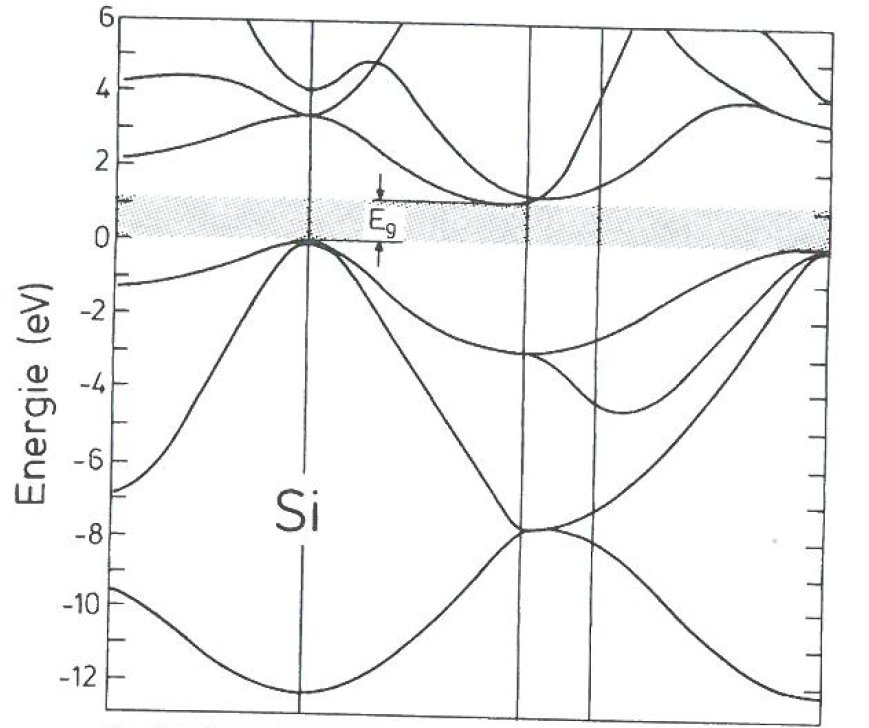
\includegraphics[angle=-1.4,scale=0.5]{Si_Bandstruktur.jpeg}\\[-3mm]
\hspace{0.8cm} L \hspace{2cm} $\Gamma$ \hspace{2.1cm} X \hspace{0.4cm} U,\,K \hspace{2cm} $\Gamma$
\caption{Bandstruktur von Si. \cite{lit:Iba09}}
\label{fig:Si_bandstructure}
\end{center}
\end{figure}
Die unteren Energiezustände fasst man als Valenzband zusammen, die oberen dagegen als Leitungsband. Zwischen diesen Bändern existiert meist eine Energielücke $E_g$, in der keine Energiezustände der Elektronen existieren können. 
Für 0 K ist das Valenzband vollständig besetzt und das Leitungsband leer, sodass praktisch kein Ladungsübertrag stattfinden kann. 
Anhand der Größe dieser Lücke kann man einen Stoff als Leiter, Halbleiter oder Isolator klassifizieren. Silizium ist ein indirekter Halbleiter, d.h. das Maximum des Valenzbandes und das Minimum des Leitungsbandes befinden sich an unterschiedlichen Punkten im $\vec{k}$-Raum. Für Raumtemperatur beträgt die Bandlücke bei Silizium 1,12 eV, für $T=0$ K ist sie etwas größer, nämlich 1,17 eV.\\
Ein Elektron im Halbleiter lässt sich in vielen Fällen wie ein freies Teilchen behandeln, wenn man die Wechselwirkung mit dem Coulomb-Potential der Atomrümpfe sowie die Wechselwirkungen mit den anderen Elektronen in eine effektive tensorielle Masse steckt. Sie ist implizit über die Komponenten des inversen Massentensors definiert und lautet wie folgt:
\begin{align}
\overline{\overline{m}}_{ij}^{-1}=\frac{1}{\hbar^2}\frac{\partial^2 E(\vec{k})}{\partial k_j \partial k_i}
\end{align}
In der Nähe des Leitungsbandminimums lässt sich $\overline{\overline{m}}^{-1}$ diagonalisieren und unter der parabolischen Näherung lautet die Energiedispersion
\begin{align}
E(\vec{k})=\frac{\hbar^2}{2}\vec{k}^\intercal\cdot \overline{\overline{m}}^{-1}\cdot \vec{k}=\frac{\hbar^2}{2}\left(\frac{1}{m_x}k_x^2+\frac{1}{m_y}k_y^2+\frac{1}{m_z}k_z^2\right)
\end{align}
In einem indirekten Halbleiter wie Silizium sind die Massen nicht gleich. Als Folge dessen sind die Flächen konstanter Energie im $\vec{k}$-Raum Rotationsellipsoide entlang einer Rotationsachse. Die effektive Masse parallel der Achse wird als \emph{longitudinale Masse} $m_l$, senkrecht dazu als \emph{transversale Masse} $m_t$ bezeichnet.\\
Für die Form des Valenzbandmaximums gelten andere Voraussetzungen, sodass sich $\overline{\overline{m}}^{-1}$ am $\Gamma$-Punkt nicht mehr diagonalisieren lässt. Die Bänder an diesem Punkt sind für die schweren und leichten Löcher (\emph{hh} bzw. \emph{lh}) entartet, zudem ergibt sich durch die Spin-Bahn-Wechselwirkung ein drittes abgesenktes Valenzband (vgl. Abbildung \ref{fig:valence_degen}).
Stattdessen lautet die Energiedispersion
\begin{align}
E(\vec{k})_{\pm}=\frac{\hbar^2}{2m_0}\left[Ak^2\pm \sqrt{B^2k^4+C^2(k_x^2 k_y^2+k_y^2 k_z^2+k_z^2 k_x^2)}\right]
\end{align}
mit den Valenzbandparametern A,B und C.
\begin{figure}[h]
\begin{center}
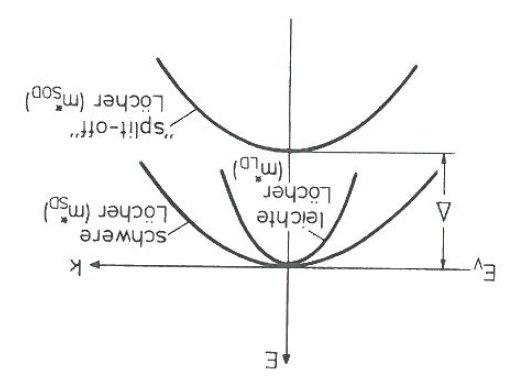
\includegraphics[angle=180,scale=0.6]{Valenzband_Entartung.jpeg}
\caption{Bandstruktur am Maximum des Valenzbandes. \cite{lit:Iba09}}
\label{fig:valence_degen}
\end{center}
\end{figure}
\subsection{Ladungsträgerdichte in intrinsischen Halbleitern}
In einem \emph{intrinsischen} Halbleiter können freie Ladungsträger nur durch thermische und photonische Anregung aus dem Valenzband in das Leitungsband gehoben werden. Bei Halbleitern ist die durch die Bandlücke $E_g$ verursachte Ladungsträgerkonzentration $n$ (Elektronen) bzw.$p$ (Löcher) stark temperaturabhängig.
Die Besetzung der elektronischen Zustände folgt der Fermi-Dirac-Verteilung
\begin{align}
f(E,T)=\frac{1}{1+\exp\left(\frac{E-\mu}{k_B T}\right)},
\end{align}
dabei ist $\mu$ das chemische Potential und $k_B$ die Boltzmann-Konstante. Für $T=0$ ist $\mu$ gleich der Fermi-Energie $E_F$, die höchstmögliche Energie welche die Elektronen im Grundzustand besitzen können.\\
Für die Berechnung der Ladungsträgerdichten werden noch die Zustandsdichten $D_C(E)$ und $D_V(E)$ im Leitungs- und Valenzband benötigt, für welche in der Nähe parabolischer Bänder gilt
\begin{align}
D_C(E)=M_C\cdot \frac{\sqrt{2m_{de}^3}}{2\pi^2\hbar^3}\sqrt{E-E_C},\hspace{1cm}
D_V(E)=\frac{\sqrt{2m_{dh}^3}}{2\pi^2\hbar^3}\sqrt{E_V-E}.
\end{align}
$E_C$ bezeichnet die Unterkante des Leitungsbands, $E_V$ die Oberkante des Valenzbands, $M_C$ steht für die Anzahl äquivalenter Leitungsbandminima. Für Silizium ist $M_C=6$, da dessen Leitungsbandminimum sich am $X$-Punkt im $\vec{k}$-Raum befindet und die sechs möglichen Raumrichtungen energetisch gleichwertig sind.\\
$m_{de}=\sqrt[3]{m_x m_y m_z}$ ist die effektive Zustandsdichtemasse für Elektronen (für Silizium ist $m_{de}=\sqrt[3]{m_l m_t^2}$) und entsprechend für Löcher gilt $m_{dh}=(m_{lh}^{3/2}+m_{hh}^{3/2})^{2/3}$.\\
Setzt man die eben eingeführten Größen in die Definitionsgleichungen 
\begin{align}
n=\int\limits_{E_C}^\infty D_C(E)\;f(E,T)\;\d E,\hspace{1cm}
p=\int\limits_{-\infty}^{E_V} D_V(E)\;[1-f(E,T)]\;\d E
\end{align}
für die Ladungsträgerkonzentrationen ein, so erhält man
\begin{align}
n=N_C\frac{2}{\sqrt{\pi}}F_{1/2}\left(\frac{E_F-E_C}{k_B T}\right),\hspace{1cm}p=N_V\frac{2}{\sqrt{\pi}}F_{1/2}\left(\frac{E_V-E_F}{k_B T}\right)
\label{eq:density1}
\end{align}
mit den effektiven Zustandsdichten
\begin{align}
N_C=2M_C\left(\frac{2\pi m_{de}k_B T}{h^2}\right)^{3/2},\hspace{1cm}N_V=2\left(\frac{2\pi m_{dh}k_B T}{h^2}\right)^{3/2}.
\end{align}
Das Fermi-Dirac-Integral $F_{1/2}$ ist definiert durch
\begin{align}
F_{1/2}(\eta_f)=\int\limits_0^\infty \frac{\eta^{1/2}\;\d \eta}{1+\exp(\eta-\eta_f)}
\end{align}
mit dem Argument $\eta_f=\frac{E_F-E_C}{k_B T}$.\\
Für $k_B T\ll E-E_F$ lässt sich die Fermi-Dirac-Statistik durch die Boltzmann-Statistik ersetzen. Dadurch ergibt sich für die Ladungsträgerkonzentrationen
\begin{align}
n=N_C\exp\left(-\frac{E_C-E_F}{k_B T}\right),\hspace{1cm} p=N_V\exp\left(-\frac{E_F-E_V}{k_B T}\right).
\label{eq:density2}
\end{align}
Das Fermi-Niveau $E_F$ stellt sich bei gegebener Temperatur so ein, dass Ladungsneutralität gegeben ist ($n=p=n_i$, $n_i$: intrinsische Ladungsträgerdichte).\\
Aus Gleichung (\ref{eq:density2}) folgt dann
\begin{align}
E_F=\frac{E_C+E_V}{2}+\frac{k_B T}{2}\ln\left(\frac{N_V}{N_C}\right)=\frac{E_C+E_V}{2}+\frac{3 k_B T}{4}\ln\left(\frac{m_{dh}}{m_{de}M_C^{2/3}}\right).
\end{align}
Die Fermi-Energie eines intrinsischen Halbleiters liegt somit etwa in der Mitte der Bandlücke $E_g$. Die intrinsische Ladungsträgerkonzentration $n_i$ ist somit
\begin{align}
n_i&=\sqrt{np}=\sqrt{N_C N_V}\exp\left(-\frac{E_g}{2k_B T}\right)\notag\\
&=4,9\cdot 10^{15}\left(\frac{m_{de}m_{dh}}{m_0^2}\right)^{3/4}M_C^{1/2}T^{3/2}\exp\left(-\frac{E_g}{2k_B T}\right)\mathrm{cm}^{-3},
\label{eq:p_intrinsic}
\end{align} 
mit der Masse $m_0$ des freien Elektrons.
\subsection{Ladungsträgerdichte im dotierten Halbleiter}
Mit Hilfe der Dotierung, dem Einbau von elektrisch aktiven Fremdatomen in einem Kristallgitter, lassen sich wesentlich höhere Ladungsträgerkonzentrationen erreichen als bei einem rein intrinsischen Halbleiter möglich wäre.\\
Die rein intrinsische Leitfähigkeit lässt sich in der Praxis kaum messen, da sie meist von einer unbeabsichtigten Dotierung induzierten Leitfähigkeit überlagert wird.\\
In einem Silizium-Kristallgitter lässt sich beispielsweise als \emph{Donator} das Element Phosphor einbauen, welches als Element der fünften Hauptgruppe im Periodensystem fünf Valenzelektronen besitzt, und somit ein Elektron zur elektrischen Leitung freigeben kann. Als möglicher \emph{Akzeptor} kann als Element der dritten Hauptgruppe Bor dienen. Dieser positive Ladungsüberschuss, im folgenden \emph{Loch} genannt, kann als Quasi-Ladungsträger innerhalb des Gitters wandern und zum Ladungsübertrag beitragen.\\
Die entsprechende Donator- und Akzeptor-Ionisierungsenergien in einem Silizium-Gitter sind für den Donator Phosphor $E_d=45$ meV bzw. für den Akzeptor Bor $E_a=45$ meV.\\
Für die Dichte $N_D^{+}$ der ionisierten Donatoren und $N_A^{-}$ der ionisierten Akzeptoren gilt
\begin{align}
N_D^{+}=\frac{N_D}{1+g_D\cdot\exp\left(\frac{E_F-E_D}{k_B T}\right)},\hspace{1cm}N_A^{-}=\frac{N_A}{1+g_A\cdot\exp\left(\frac{E_A-E_F}{k_B T}\right)},
\label{eq:don_acc_density}
\end{align}
dabei ist $N_D$ bzw. $N_A$ die Dichte aller Donatoren bzw. Akzeptoren und $E_D$ bzw. $E_A$ die absolute Energie eines gebundenen Donatorelektrons bzw. Akzeptorlochs. Außerdem gelten für die Degenerationsfaktoren $g_D=2$ für Donatoren und $g_A=4$ für Akzeptoren. Wie beim intrinsischen Halbleiter stellt sich die Fermi-Energie so ein, dass Ladungsneutralität vorherrscht. Die Abbildung \ref{fig:fermi_dot} zeigt das schematische Banddiagramm, die Zustandsdichte, die Fermi-Dirac-Verteilung und die Ladungsträgerkonzentration für einen intrinsischen, einen $n$- und einen $p$-dotierten Halbleiter.\\
\begin{figure}
\centering
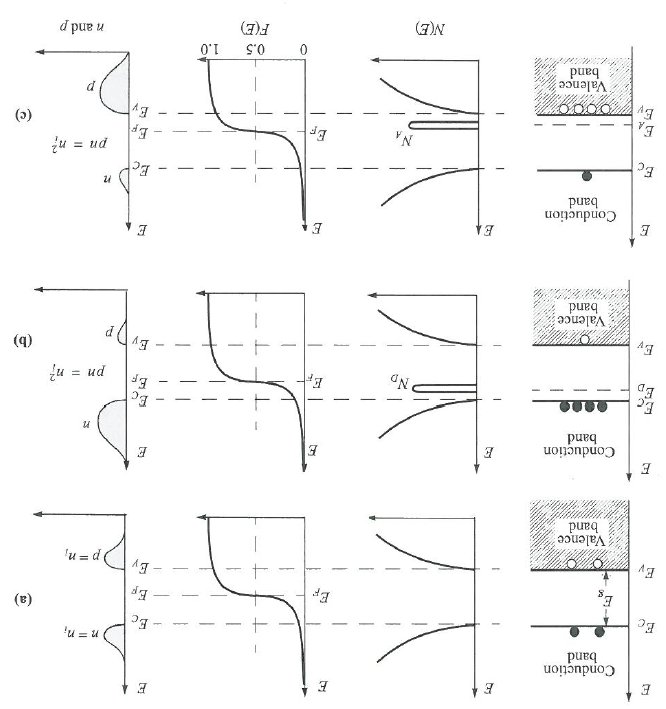
\includegraphics[angle=180,scale=0.9]{Fermi_dot.jpeg}
\caption[Banddiagramm, Zustandsdichte, Fermi-Dirac-Verteilung, Ladungsträgerkonzentration]
{Schematisches Banddiagramm, Zustandsdichte, Fermi-Dirac-Verteilung und Ladungsträgerkonzentration für einen (a) intrinsischen ,(b) $n$-dotierten und (c) $p$-dotierten Halbleiter im thermischen Gleichgewicht. \cite{lit:Sze07}}
\label{fig:fermi_dot}
\end{figure}
Für eine reine $p$-Dotierung gilt
\begin{align}
p=N_A^{-}+n
\end{align}
und somit in Boltzmann-Näherung mit (\ref{eq:density2}) und (\ref{eq:don_acc_density}) folglich
\begin{align}
N_V\exp\left(-\frac{E_F-E_V}{k_B T}\right)=\frac{N_A}{1+g_A\cdot\exp\left(\frac{E_A-E_F}{k_B T}\right)}+N_C\exp\left(-\frac{E_C-E_F}{k_B T}\right).
\end{align}
Die Fermi-Energie kann numerisch aus dieser impliziten Gleichung ermittelt werden.\\
Für einen Temperaturbereich, in dem die intrinsische Ladungsträgerkonzentration keine Rolle spielt, d.h. $p=N_A^{-}$, folgt aus (\ref{eq:density2}) und (\ref{eq:don_acc_density}) die implizite Gleichung
\begin{align}
p\approx\frac{N_A}{1+g_A\frac{p}{N_V}\exp\left(\frac{E_a}{k_B T}\right)}
\end{align}
mit $E_a=E_A-E_V$. Aufgelöst nach $p$ ergibt sich
\begin{align}
p\approx 2N_A\left[1+\sqrt{1+4g_A\frac{N_A}{N_V}\exp\left(\frac{E_a}{k_B T}\right)}\right]^{-1}.
\label{eq:density_p}
\end{align}
Man spricht von einer \emph{Störstellenreserve}, wenn bei niedrigen Temperaturen ($k_B T\ll E_a$) viele Akzeptoren noch nicht ionisiert sind. So vereinfacht sich \eqref{eq:density_p} zu
\begin{align}
p\approx \frac{1}{2}\sqrt{N_A N_V}\exp\left(-\frac{E_a}{2k_B T}\right).
\label{eq:p_approx}
\end{align}
Für genügend hohe Temperaturen, wenn praktisch alle Störstellen ionisiert sind, spricht man dann von einer \emph{Störstellenerschöpfung} und es folgt
\begin{align}
p\approx N_A.
\end{align}
Die Temperaturabhängigkeit der Ladungsträgerkonzentration $n$ in einem $n$-dotierten Silizium ist in Abbildung \ref{fig:si_density_temp} zu sehen. Für $p$-dotiertes Silizium ist der qualitative Verlauf weitgehend identisch; er unterscheidet sich lediglich um einige Faktoren.
\begin{figure}[p]
\centering
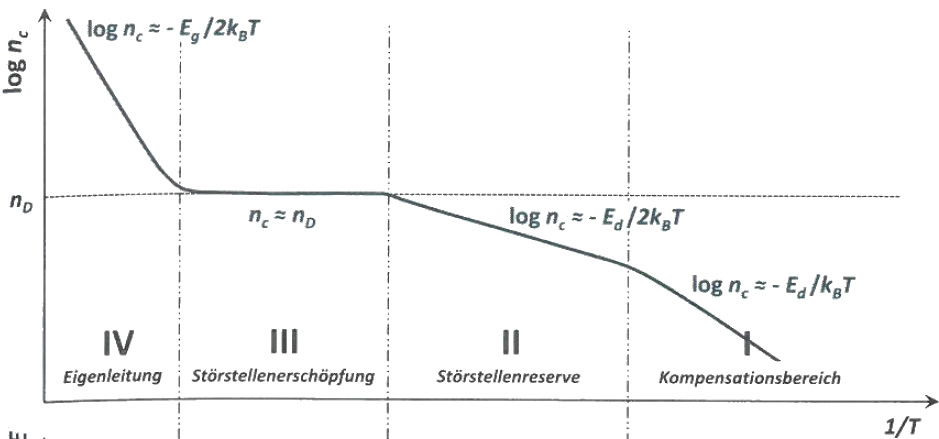
\includegraphics[scale=0.6]{Si_density_temp_n.jpeg}
\caption{Qualitative Abhängigkeit der Ladungsträgerkonzentration in einem n-dotierten Halbleiter von der Temperatur. \cite{lit:GroMa14}}
\label{fig:si_density_temp}
\end{figure}
Bei sehr hohen Temperaturen dagegen dominiert die intrinsische Ladungsträgerkonzentration $n_i$. Die \emph{intrinsische Temperatur} $T_i$ ist die Temperatur, bei der die intrinsische Ladungsträgerkonzentration $n_i$ gleich der durch eine Dotierung verursachte Ladungsträgerdichte ist. %Sie ist in Abbildung \ref{fig:intrin_temp} für Silizium dargestellt. 
In Abbildung \ref{fig:fermi_density} ist die Fermi-Energie von Silizium als Funktion der Temperatur und der Störstellenkonzentration veranschaulicht.
%\begin{figure}[h]
%\centering
%%\includegraphics[scale=1]{Intrin_Temp.pdf}
%\caption{Intrinsische Temperatur als Funktion der Störstellenkonzentration. \cite{lit:Sze07}}
%\label{fig:intrin_temp}
%\end{figure}
\begin{figure}[p]
\centering
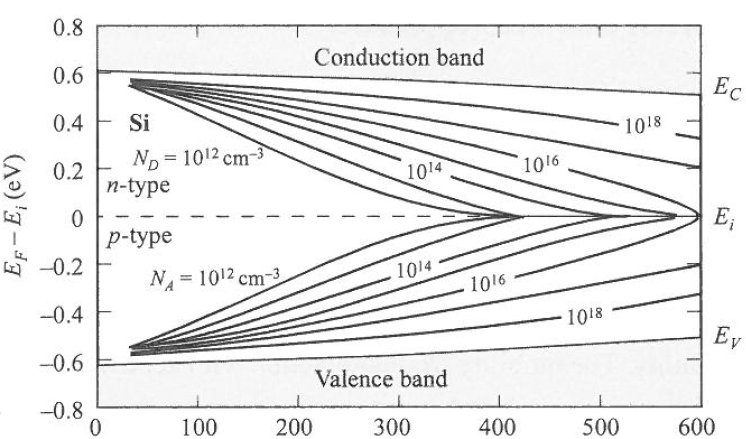
\includegraphics[scale=0.7]{Fermi_Density.jpeg}
\caption{Fermi-Energie von Silizium als Funktion der Temperatur und der Störstellenkonzentration. \cite{lit:Sze07}}
\label{fig:fermi_density}
\end{figure}
\subsection{Bewegung von Ladungsträgern in elektromagnetischen Feldern}
Das Drude-Modell des freien Elektronengases lässt sich auch auf Halbleiter anwenden. In einem äußeren elektrischen Feld $E$ lautet die Bewegungsgleichung des Lochs in einem Halbleiter
\begin{align}
m\frac{\d v}{\d t}+\frac{m}{\tau}v_d=eE,
\end{align}
hierbei ist $e$ die Elementarladung und $v_d=v-v_\text{therm.}$ die \emph{Driftgeschwindigkeit}, welche abhängig von der zu bewegenden Ladung parallel oder antiparallel zum elektrischen Feld ist.
Es ist zu beachten, dass $v_d$ eine Netto-Geschwindigkeit der Ladungsträger in einem äußeren Feld ist, und somit als ein Erwartungswert betrachtet werden muss.
Der Term $mv_d/\tau$ stellt einen durch Stößen an akustischen Phononen oder Gitterdefekten verursachte Reibung dar. Die \emph{Relaxationszeit} $\tau$ stellt mikroskopisch die mittlere Zeit zwischen zwei aufeinanderfolgenden Stößen dar.\\
Im stationären Fall gilt dann
\begin{align}
v_d=\frac{e\tau}{m}E=\mu E
\end{align}
mit der \emph{Beweglichkeit}
\begin{align}
\mu=\frac{e\tau}{m}.
\end{align}
Für die Stromdichte $j$ in Feldrichtung erhält man
\begin{align}
j=epv_d=ep\mu E,
\end{align}
woraus mit dem Ohmschen Gesetz
\begin{align}
j=\sigma E
\end{align}
für die elektrische Leitfähigkeit folgt:
\begin{align}
\sigma=ep\mu=e^2p\tau/m.
\end{align}
Der \emph{spezifische Widerstand} als Kehrwert der Leitfähigkeit ist folglich
\begin{align}
\rho=\sigma^{-1}=(ep\mu)^{-1}.
\label{eq:p_rho_mu}
\end{align}
Die Streuung von Ladungsträgern an akustischen Phononen und an geladenen Störstellen stellen die größten Beiträge zur Relaxationszeit $\tau$ und somit   zur Beweglichkeit $\mu$.\\
Für tiefe Temperaturen nimmt die Beweglichkeit mit $T^{3/2}$ zu, da die zunehmende thermische Geschwindigkeit der freien Ladungsträger zu einer geringeren Ablenkung an den geladenen Störstellen führt. Dagegen werden bei höheren Temperaturen immer mehr akustische Phononen erzeugt, an denen die Ladungsträger gestreut werden. In dem Temperaturbereich nimmt die Beweglichkeit mit $T^{-3/2}$ ab. Diese Temperaturabhängigkeit der Beweglichkeit ist in der Abbildung \ref{fig:mu-temp_dep} veranschaulicht.

Setzt man die Ladungsträger neben dem elektrischen Feld $\vec{E}$ noch einem magnetischen Feld $\vec{B}$ aus, so erhalten die Leihfähigkeit $\sigma$ und der spezifische Widerstand $\rho$ tensoriellen Charakter.
\enlargethispage{3em}
\begin{figure}[h!]
\centering
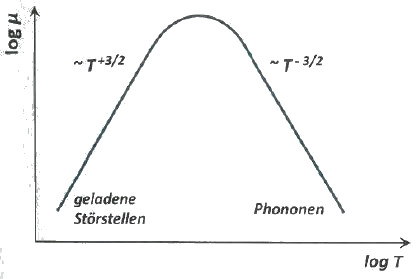
\includegraphics[scale=0.8]{Mu_temp_dep.jpeg}
\caption{Temperatur-Abhängigkeit der Beweglichkeit $\mu$ in Halbleitern. \cite{lit:GroMa14}}
\label{fig:mu-temp_dep}
\end{figure}

\newpage
\subsection{Hall-Effekt}
Man betrachtet eine quaderförmige homogene Halbleiterprobe (\emph{Hall bar}), welche in $x$-Richtung von einem konstanten Strom durchflossen wird. Zudem wird in $z$-Richtung ein homogenes $B$-Feld angelegt. Die schematische Anordnung ist in Abbildung \ref{fig:hall-effect} zu sehen.
\begin{figure}[h]
\centering
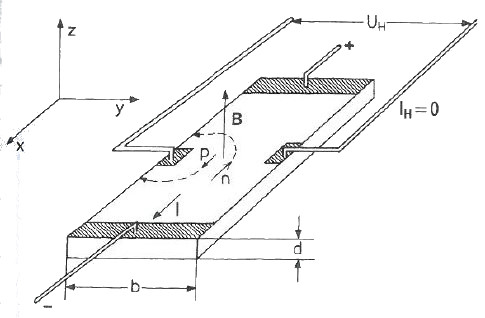
\includegraphics[scale=1]{Hall_effect.jpeg}
\caption{Schematische Anordnung einer Hall-Messung. \cite{lit:Iba09}}
\label{fig:hall-effect}
\end{figure}

In der Annahme, dass der Stromfluss nur in $x$-Richtung möglich ist ($j_x=j$), folgt für p-Leitung
\begin{align}
E_y=\frac{1}{pe}Bj=R_H B\frac{I}{bd}.
\end{align}
In $y$-Richtung baut sich folglich ein elektrisches Feld, das \emph{Hall-Feld} auf, und somit entsteht eine Hall-Spannung mit
\begin{align}
U_H=E_y\cdot b=R_H B I\frac{1}{d}.
\end{align}
Mit der sogenannten \emph{Hall-Konstante} $R_H=1/pe$ kann somit bei bekannter Probendicke $d$, den Magnetfeld $B$, der Stromstärke $I$ und der Hall-Spannung $U_H$ die Ladungsträgerdichte $p$ bestimmt werden.

\newpage
Die Beweglichkeit $\mu$ der Ladungsträger erhält man aus der Längsspannung
\begin{align}
U_x=E_x\cdot l=\frac{1}{ep\mu}I\frac{l}{bd}
\end{align}
über die Länge $l$ der Probe.

Für eine nicht-quaderförmige Probengeometrie kann ebenfalls die Ladungsträgerdichte $p$ und die Beweglichkeit $\mu$ ermittelt werden. Dazu hat L.J. van der Pauw eine Methode beschrieben, welche im folgenden Abschnitt näher erläutert wird.
\subsection{Van-der-Pauw-Methode}
An einem planparallelen Plättchen (vgl. Abbildung \ref{fig:vdP}) werden am Rand vier kleine Kontakte M,N,O und P angebracht. Zwischen M und N lässt man einen elektrischen Strom $I_\text{MN}$ fließen und misst den Spannungsabfall $U_\text{P}-U_\text{O}$ zwischen den Kontakten O und P.
\begin{figure}[h]
\centering
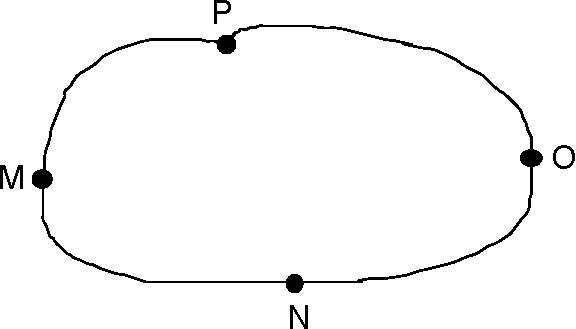
\includegraphics[scale=1]{arbitrary_plate.pdf}
\caption{Planparalleles Plättchen mit der Dicke $d$ und beliebiger Form mit vier Kontakten M,N,O und P am Rand.}
\label{fig:vdP}
\end{figure}

 Damit erhält man den Widerstand
\begin{align}
R_\text{MN,OP}=\frac{U_\text{P}-U_\text{O}}{I_\text{MN}}
\end{align}
und analog
\begin{align}
R_\text{NO,PM}=\frac{U_\text{M}-U_\text{P}}{I_\text{NO}}.
\end{align}
Zwischen den Widerständen $R_\text{MN,OP}$ und $R_\text{NO,PM}$ besteht folgende Beziehung
\begin{align}
\exp\left(-\frac{\pi d}{\rho}R_\text{MN,OP}\right)+\exp\left(-\frac{\pi d}{\rho}R_\text{NO,PM}\right)=1,
\end{align}
wobei $d$ die Dicke und $\rho$ der gesuchte spezifische Widerstand der scheibenförmigen Probe ist. Diese implizite Gleichung lässt sich numerisch nach $\rho$ auflösen.

Eine andere Möglichkeit ist, den spezifischen Widerstand mit der Gleichung 
\begin{align}
\rho=\frac{\pi d}{\ln 2}\frac{R_\text{MN,OP}}{R_\text{NO,PM}}
\end{align}
zu berechnen, wobei $f$ eine Größe ist, die nur von dem Quotienten
\begin{align}
Q=\frac{R_\text{MN,OP}}{R_\text{NO,PM}}
\end{align}
abhängt. Sie ist implizit über die Gleichung
\begin{align}
\cosh\left(\frac{Q-1}{Q+1}\cdot\frac{\ln 2}{f}\right)=\frac{1}{2}\exp\left(\frac{\ln 2}{f}\right)
\end{align}
definiert, diese sei in Abbildung \ref{fig:f(Q)} als Funktion von $Q$ veranschaulicht.
\begin{figure}[h]
\centering
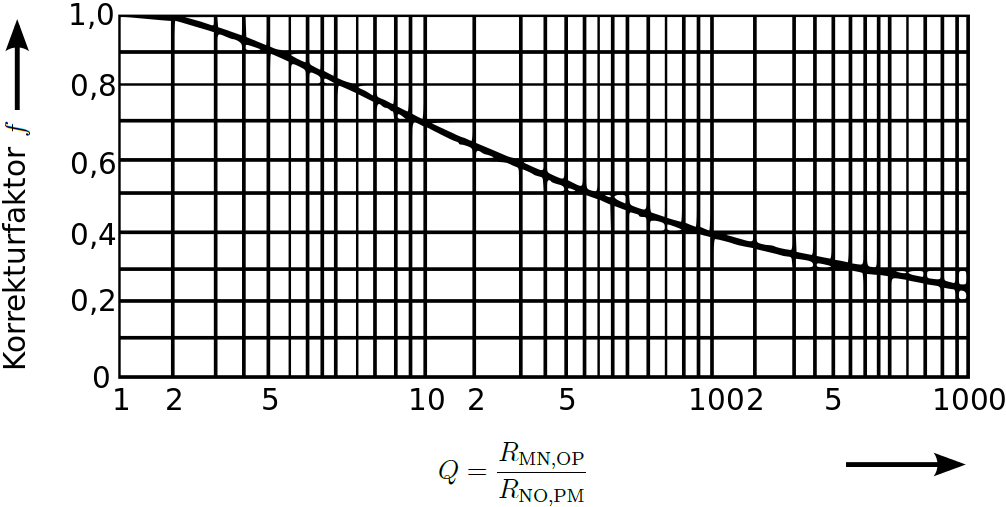
\includegraphics[width=0.9\textwidth]{Pauw_Korrektur.png}
\caption{Korrekturfaktor $f(Q)$ zur Berechnung des spezifischen Widerstands $\rho$. \cite{lit:Wiki1}}
\label{fig:f(Q)}
\end{figure}

\newpage
Möchte man nun die Ladungsträgerkonzentration über den Hall-Effekt bestimmen, so leitet man einen Strom $I_\text{MO}$ zwischen zwei nicht aufeinanderfolgenden (sie müssen nicht zwangsläufig gegenüber liegen) Kontakten. Dann bestimmt man wie bei der Berechnung des spezifischen Widerstands $\rho$ im vorherigen Abschnitt den Widerstand $R_\text{MO,NP}$. Schaltet man nun ein homogenes Magnetfeld $B$ senkrecht zur Probe zu, so ändert sich der Widerstand um den Betrag $\Delta R_\text{MO,NP}$.
Unter der Voraussetzung, dass
\begin{enumerate}
\item die Kontakte hinreichend klein sind und sich am Rand der Probe befinden;
\item die Probe in der Dicke homogen ist und keine Löcher enthält,
\end{enumerate}
lässt sich die Hall-Konstante $R_H$ definieren durch
\begin{align}
R_H=\frac{d}{B}\Delta R_\text{MO,NP}.
\end{align}
Diese Gleichung ist insofern gültig, da das Stromlinienfeld nicht vom außen angelegten Magnetfeld beeinflusst wird. Dies gilt für jede beliebige Probengeometrie sofern obige Bedingungen erfüllt sind.

Für das elektrische Feld gilt die Relation
\begin{align}
\vec{E}=\frac{1}{\mu}\vec{v}_d\times \vec{B}=\frac{1}{ep\mu}\vec{j}-\frac{1}{ep}(\vec{j}\times \vec{B})=\vec{E}_{\parallel}-\vec{E}_{\perp},
\end{align}
d.h. das elektrische Feld, beeinflusst vom Magnetfeld, lässt sich in einem Anteil parallel und senkrecht zum Stromlinienfeld aufteilen. Berechnet man nun die Hall-Spannung quer zur Probe, bspw. von P nach N (vgl. Abbildung \ref{fig:current_field}), so gilt

\begin{align}
U_\text{PN}&=\int\limits_{\mathrm{P}}^{\mathrm{N}}\vec{E}\;\d \vec{s}
=\int\limits_{\mathrm{P}}^{\mathrm{N}^\prime}-\frac{1}{ep}(\vec{j}\times \vec{B})\;\d\vec{s}
+\underbrace{\int\limits_{\mathrm{N}^\prime}^{\mathrm{N}}\frac{1}{ep\mu}\vec{j}\;\d \vec{s}}_{=:\, U_\text{offset}}\notag\\
&=-\frac{1}{ep}\int\limits_{\mathrm{P}}^{\mathrm{N}^\prime}|\vec{j}\times\vec{B}|\;\d s  +  U_\text{offset}
=-\frac{B}{ep}\int\limits_{\mathrm{P}}^{\mathrm{N}^\prime}j\;\d s  +  U_\text{offset}\notag\\
&=-\frac{B}{ep}\int\limits_{\mathrm{P}}^{\mathrm{N}^\prime}\frac{\d I}{d}  +  U_\text{offset}
=-\frac{B}{epd}\underbrace{\int\limits_{\mathrm{P}}^{\mathrm{N}^\prime}\d I}_{I}  +  U_\text{offset}\notag\\
&=-\frac{B}{epd}\cdot I +U_\text{offset}=-R_H\frac{BI}{d}+U_\text{offset}
\label{eq:U_offset}
\end{align}
Somit misst man bei der Hall-Spannung immer eine Offset-Spannung mit. Diese lässt sich aber durch die Messung der Hall-Spannung mit entgegengesetzten Strom und anschließender Subtraktion der Spannungen eliminieren.

\begin{figure}[h]
\centering
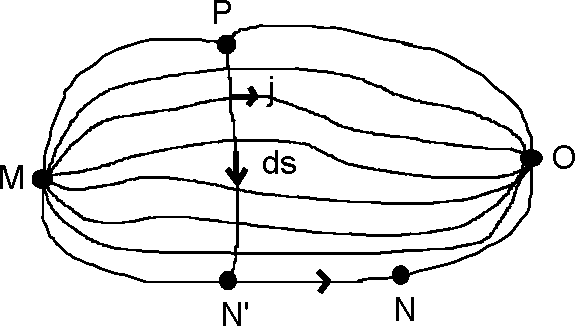
\includegraphics[scale=1]{current_field.pdf}
\caption[Stromlinienfeld innerhalb der planparallelen Probe.]{Stromlinienfeld innerhalb der planparallelen Probe. Die Integrationswege von P über N' nach N ergeben die elektrischen Feldkomponenten.}
\label{fig:current_field}
\end{figure}

% !TeX encoding = UTF-8
% !TeX root = V7_Lichtbeugung.tex
% !TeX spellcheck = de_DE_frami



%\textsf{He-Ne}-Laser mit Wellenlänge $\lambda=633$\,nm
%Linse $L_1$ mit Brennweite $f_1=199\pm2$\,mm
%Linse $L_2$ mit Brennweite $f_1=151\pm2$\,mm
%CCD-Kamera mit Pixeln der Größe $9\,\micro\metre \times 9\,\micro\metre$


% \usepackage[free-standing-units]{siunitx}
% \sisetup{locale = DE}					% fuer deutsche Dezimaltrenner und Aufzaehlungen
% \DeclareSIUnit\px{px}

\section{Auswertung}

\subsection{Versuchsaufbau und Versuchsziele}

\begin{figure}[h]
\centering
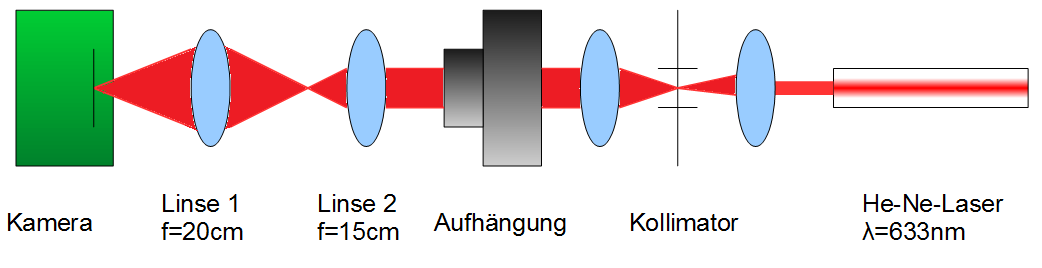
\includegraphics[width=\textwidth]{versuchaufbau.png}
\caption[Versuchsaufbau]{Schematische Darstellung des Versuchsaufbaus. Der Strahl eines Helium-Neon-Lasers (\textsf{He-Ne}-Laser) wird mit Hilfe eines Kollimators zu einer Punktquelle begrenzt, aufgeweitet und parallelisiert. Hierzu besteht der Kollimator aus zwei bikonvexen Linsen und einer Lochblende, welche zwischen den Linsen positioniert ist. Die erzeugten parallelen Strahlen durchlaufen eine Aufhängung, in welche verschiedene Objekte eingesetzt werden können. Für die Beugungsmuster im Fourierraum wird nur Linse 1 mit Brennweite $f_1=20\,\centi\metre$ benutzt, dessen Fourierebene direkt auf dem Detektionsmedium liegt. Für eine echte Abbildung wird Linse 2 mit $f_2=15\,\centi\metre$ zwischen Linse 1 und Aufhängung platziert.}
\label{aufbau}
\end{figure}

Der Versuchsaufbau, welcher für den Versuch Lichtbeugung benötigt wird, ist schematisch in Abbildung \ref{aufbau} illustriert. Die benötigte photonische Einstrahlung basiert auf einem Helium-Neon-Laser mit einer Wellenlänge $\lambda=633\,\nano\metre$. Im Strahlengang wird ein Kollimator positioniert, um aus einem kontinuierlichen Laserstrahl eine Punktquelle zu erzeugen. Mit Hilfe der zweiten Kollimator-Linse wird ein paralleler Strahlengang hergestellt. Weiter werden bis auf die erste Beugungsordnung der Blende alle höheren Ordnungen durch die Aufhängung ausgeblendet. Für die Bildgebung (genauer: echte und Fourier Abbildung) wird nun diese zentrale Ordnung durch das Objekt geleitet. Die montierten Bilder, außer Einstein- und Bikini Model-Bild, können schematisch in der nächsten Abbildung \ref{Masken} gesehen werden.

\begin{figure}[h]
\centering
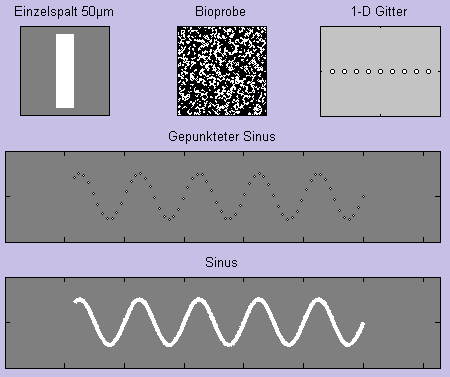
\includegraphics[width=0.95\textwidth]{Masken.png}
\caption[Maskenformen]{Schematische Darstellung der montierten Bildmasken}
\label{Masken}
\end{figure}

Im Rahmen des Experiments sind drei Messung durchgeführt worden. Dabei wurden die Brennweiten der Linsen (1) und (2) überprüft. Weiter wurde die Spaltbreite eines Einzelspaltes bestimmt und zuletzt Beugungsbilder sowie Abbildungen der Masken in Abbildung \ref{Masken} aufgenommen.

Zu Beginn des Experiments wurde eine komplette Neu-Justierung des Systems vorgenommen, da bei einer schlechten Justage u.a. die Brennweitenbestimmung der Linsen (1) und (2) durch optische Fehlerquellen ungenau wird. Die erhaltenen Brennweiten sind in der nachfolgende Tabellen (\ref{Brennweite}) eingetragen.

\begin{table}[hb]
	\centering
	\caption[]{Resultate der Brennweiten Bestimmung}
	\begin{tabular}{ccc}
		\toprule
				& Brennweite $f$ in mm 	& 	Fehler in mm	\\
		\midrule
		Linse 1	& 199				&	$\pm1$		\\
		Linse 2	& 151				&	$\pm2$		\\
		\bottomrule
	\end{tabular}
	\label{Brennweite}
\end{table}

Die Messresultate sind überraschend gut und bedürfen keiner weiteren Diskussion.
% Allerdings ist zu erwähnen, dass bei früher Messungen die Brennweiten nicht mit der Herstellerangabe übereinstimmten. Es wurde herausgefunden, dass dieser Effekt durch schlechte Justierung hervorgerufen wird. Dieses Problem genügt einer simplen Erklärung. Bei schlechter justage wird sphärische Abberation und dadurch eine Brennweiten Verfälschung erzeugt, bezogen auf Brennweite Messungen mit monochromatischen und paraxialen Wellen.

\section{Spaltbreitenbestimmung} \label{Spaltbreitenbestimmung}
Die zweite Aufgabe im Experiment ist die Spaltbreiten Bestimmung eines Einzelspaltes. Zu diesem Zweck dient die Intensitätsverteilung des Einzelspalt Beugungsbilds in Abbildung \ref{ESpaltBeugung} und Formel \eqref{eq:Messung}.
\begin{figure}[h]
\centering
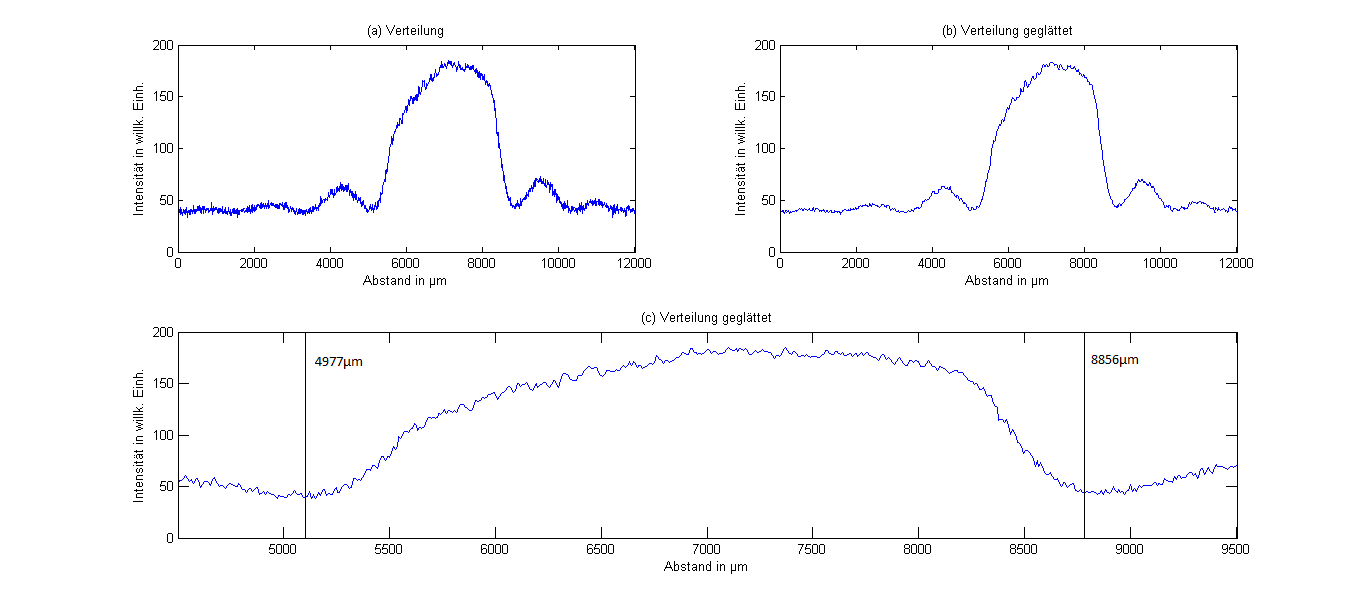
\includegraphics[width=\textwidth]{verteilung.png}
\caption[Intensitätsverteilung]{Intensitätsverteilung bei Beugung an einem Einzelspalt. Es zeigt, wie erwartet, den Verlauf eines Sinus Cardinalis. Die Position null µm gibt einen Rand des Chips an. Abbildung (a) illustriert die unbearbeiteten Daten. In Abbildung (b) wurde die Kurve geglättet. Abbildung (c) ist eine Vergrößerung von (b) um die erste Beugungsordnung.}
\label{ESpaltBeugung}
\end{figure}

Bekannten Messparameter sind die Wellenlänge $\lambda=633~\mathrm{nm}$ und der Abstand vom Spalt zum Schirm $s=35~cm\pm~\mathrm{1mm}$. Mit Hilfe der Intenistätsverteilung aus \ref{ESpaltBeugung} ergibt sich die Breite des ersten Maximum mit $b=3,879~\mathrm{mm}\pm 0,05~\mathrm{mm}$. Mit Hilfe der Gleichung \eqref{eq:Messung} ergibt sich eine Spaltbreite von $d=60~\mathrm{\mu m}\pm80~\mathrm{\mu m}$. Der errechnete Wert beträgt nicht gerundet $57\mathrm{\mu m}$ und liegt in der Nähe der Angabe des Herstellers von $50~\mathrm{\mu m}$. Problematisch ist der berechnete Fehler. Dieser Umstand hat einen simplen Grund. Die beiden ersten Minimas um den ersten Maximum wurden improvisorisch mit Hilfe eines Matlab Skriptes bestimmt. Das Problem bei diesem Verfahren ist das Rauschen im Signal. Dabei kann es vorkommen, dass ein versetztes Minimum gefunden wird. Deshalb wurde hier der Fehler auf $50~\mathrm{\mu m}$ geschätzt und der berechnete Fehlerwert kann vernachlässigt werden.

\section{Fourier-Beugungen und echte Abbildungen}
Die letzte Aufgabe war die Erstellung von Beugungsbildern sowie echte Abbildungen der in Abbildung \ref{Masken} gezeigten Masken. Im folgenden werden die einzelnen Bilder vorgeführt und relativ kurz darüber diskutiert. Dabei wird die Reihenfolge echte Abbildung und Beugungsbild bei jeder einzelner Maske eingehalten.
\paragraph{Einzelspalt} Das durch die Vorlesung bekannte Muster eines Einzelspaltes wurde auch hier beobachtet. Dabei ist die Stellung des Spaltes in der Maske vertikal. Die horizontale Anordnung der Intensitätsverteilung im Beugungsbild (Fourierraum) entspricht der Theorie. Beide gemessene Bilder ergänzen sich zu einander. Dabei wurde in der echten Abbildung das Hintergrundrauschen nicht abgezogen, da diese die qualitativen Analyse nicht behindert. Im Beugungsbild wurde allerdings eine art exponentielle Krümmung beobachtet. Qualitativ kann dieser Fehler durch eine spährische Abberration und/oder ein schiefer Einfall in die Optik erklärt werden, da im Experiment eine nicht paraxialer Strahl benutzt wurde. Ebenso erkennt man eine auf der rechten Seite im Beugungsbild eine Aufspaltung des Maximas in zwei Linien. Diese Erscheinung ist nicht trivial. Der erste Erklärungsversuch wäre diese Linien als ein Resultat eines Diodenlaser zu sehen, da solche Laser einen ähnlichen Verlauf zeigen. Allerdings wurde im Experiment eine Gasentladungslaser benutzt. Eine weitere Erklärung wären, dass durch die eingestellte Optik zwei verschiedene Niveaus abgebildet wurden, wobei diese Aufgabe nicht trivial ist. Falls dies hier eingetreten ist kann dies nur aus purem Zufall eingetreten sein.

\paragraph{Bio-Probe} Weiter wurde eine Probe mit unbekannter Struktur und Materie untersucht, die hier Bio-Probe getauft wurde. Die echte Abbildung zeigt eine Vergrößerung an einem Punkt der Maske. Es sind vereinzelte Strukturen zu erkennen. Allerdings ist hier nicht klar, ob die Struktur in der Maske oder auf der Öberfläche sich befindet. Es kann nicht ausgeschlossen werden, dass die gemessenen Strukturen einfache Schmutzansammlungen auf der Oberfläche sind. Das Beugungsbild ist ebenso unbefriedigend. In Fourierraum wurden neben dem gezeigten Hauptmaximum, in Richtung diagonal rechts/oben ein weiteres INterferenzmaximum mit dem bloßen Auge beobachtet. Allerdings ist der direkte Abstand zu groß um beide in der Kamera zu erfassen. Daher wird nur das Hauptmaximum gezeigt. Ersichtlich ist eine konstruktive Interferenz nur am Laserspot.

\paragraph{1-D Gitter} Ein weiteres bekanntes Bild ist das ein Eindimensionale Gitter. Dabei entspricht die echte Abbildung dem Beugungsbild. Durch horizontale Anordnung der Punkte zu einem Gitter, werden alle horizontalen Interferenzen zu einander aufgehoben. Dabei überleben nur die vertikalen Interferenzen. Es ist theoretisch möglich die Lochgröße mit dem Beugungsbild zu bestimmen. Dies würde auf analogerweise, wie eine Spaltbreitenbestimmung eines Einzelspaltes geschehen. Es wurde allerdings im Rahmen des Experimentes nicht durchgeführt.

\paragraph{gepunkteter Sinus} Eine gepunktete Sinuskurve diente als Maske. Dabei ist das Beugungsbild sehr Interessant und erzeugt eine völlig unterschiedliche Struktur verglichen mit einem durchgehenden Sinus, welcher weiter im nächsten Paragraphen diskutiert wird. Das Beugungsbild zeigt im Zentrum mehrere zu einander verschobene kantige Sinusverläufe. Weiter außerhalb sind zwei in ihrer Intensität relativ schwache Beugungsringe zu beobachten. Verglichen mit einzelnen Messungen - jetzt im Gedankengang eine einzelne kleine Blende - sind diese Interferenzringe ein Effekt der einzelnen Punkte (oder auch im entfernten Sinne "Blende"). Das Zentrum des Beugungsbildes ist eine intensive Überlagerung der Sinusstruktur und vieler einzelner Punkte/Blenden. Mathematisch lässt sich bei einem Sinusverlauf die Differenz zweier Dirac-Distributionen, in der Form

\begin{equation}
	\mathcal{FT}(sin(x))=\frac{1}{i}(\delta(x-\omega_0)-\delta(x+\omega_0))~\mathrm{,}
\end{equation}
berechnen. Dies findet man im Beugungsbild. Man nehme sich einen hellen Punkt im Beugungsbild und laufen in horizontaler/vertikaler Richtung bis zu nächsten hellen Punkt. Diese beiden Punkte entsprechen dem positiven Beitrag der Dirac-Distribution. Die schwarze Punkt in der Mitte ist der negative Beitrag zur ersten Distribution. Theoretisch ist es möglich die Verschiebung $\omega_0$ durch die Distanz zwischen erster hellen und erster dunkel Distribution zu berechnen. Dabei ist eine Intensitätsverteilung, wie in \ref{Spaltbreitenbestimmung}. Allerdings wurde dies im Rahmen des Experiments nicht bestimmt.

\paragraph{Sinus} Zum weiteren Vergleich dient eine kontinuierliche Sinusform. Die Ergebnisse der Sinus Maske ist eine Vergrößerte Abbildung der Maske und das dazugehörige Beugungsbild. Aus der echten Abbildung ist eine nicht kontinuierlicher Sinus, sowie an einer Stelle eine Deformation im Verlauf ersichtlich. Für weitere Analysen wird an dieser Stelle ein kontinuierlicher Sinus angenommen. Das Beugungsbild gibt eine sehr schöne experimentelle Ergänzung zur Fourier Transformierten des Sinus. Dabei sind zwei gekreuzte Geraden zu erkennen. Jede dieser einzelnen Geraden kann zu einem Ergebnis eines Einzelspaltversuches aufgeteilt werden. Dabei erkennt man pro Gerade einen periodischen Wechsel zwischen Maxima und Minima. Dabei ist das Zentrum des Beugungsbildes eine Intensitätsüberlagerung beider Geraden. Des Weiteren ist hier genauso die mathematische Beschreibung des Fourier Transformierten Sinus wiederzufinden. Der imaginäre Faktor $i$ tritt durch die Winkeldrehung in Erscheinung.

\paragraph{Bikini-Model} Der Masken Favorit war die Bikini-Model Maske. Dabei wurde eine nicht schöne Abbildung erstellt, dafür ein besseres Beugungsbild. In der echten Abbildung musste etwas getrickst werden um eine relativ deutliche Abbildung zu messen. Die Abbildung erfolgte mit einer Distanz Verkürzung zwischen Kamera und der Linse (1), da bei theoretisch geforderten Positionierung nicht genug Intensität erhalten wurde. Ersichtlich ist die zu abbildende Bikini-Model und schiefe Streifen, welche Herstellungsbedingt sein sollten. Im Beugungsbild sind neben dem Hauptmaximum im Zentrum weitere gitterförmig angeordnet Punkte zu erkennen. Dabei ist nicht ganz klar, ob diese wirklich von den schiefen Streifen in der echten Abbildung kommen. Verglichen mit einem zwei Zweidimensionalen Beugungsgitter müssten die Struktur im Beugungsbild um einen bestimmten Winkel gedreht sein, da die Streifen in der echten Abbildung ebenfalls einen Winkel zu einer Achse aufzeigen. Daher ist es nicht auszuschließen, dass diese Winkelverschiebung bei einer Überlagerung mit einer relativ hübschen Frau in Bikini diese Winkeldrehung verschwindet. Interessant wäre eine Messung mit dem gleichen Bild mit dem Unterschied, dass diese Streifen in einem anderen Winkel auftreten. Weiter sieht man im Beugungsbild einen Abbildungsfehler. Die Beugungsordnungnen am rechten Rand weisen Koma artige Erscheinungen auf.

\paragraph{Einstein} Die letzte verwendete Maske ist das bekannte Einstein Beugungsporträt. Es wurde eine vergrößerte Version der Abbildung erstellt, wobei man Konturen und Gesichtszüge relativ gut erkennen kann. Das Beugungsbild entspricht der bekannten Form. Die Überlagerung von Gitterinformation und Bildinformation ist sehr gut zu erkennen. Dabei entsprechen alle intensiven Ordnungen Bildinformationen. Die zusätzlich auftretende Linienförmige Intensitätsverteilung entspricht einer horizontalen Gitterstruktur in der Maske. Weiter ist am Rande ein Abbildungsfehler der Art Koma zu erkennen. Weiter kann mit einer weiteren Blende zwischen Linse (1) und (2) die Dunkelfeldmethode bzw. Hellfeldmethode durchgeführt werden. Dabei würde bei ersteren die Konturen im Bild viel besser zu Geltung kommen. Die experimentelle Realisierung würde durch die weitere Blende stattfinden. Phänomenologisch würde man alle Ordnungen ausblenden bis auf hier einer der vier zweiten Beugungsordnungen. Analog die Hellfeldmethode besitzt sehr viel Intensität im Bild. Diese Methode betont weniger die Konturen im Bild. Erzeugt wird dieses Phänomen ebenfalls mit einer Blende, wobei nur das erste Hauptmaximum nicht ausgeblendet wird. Die Blende ist ebenfalls zwischen der Fourier- und der Abbildungslinse.


\newpage
\begin{figure}[h]
	\centering
	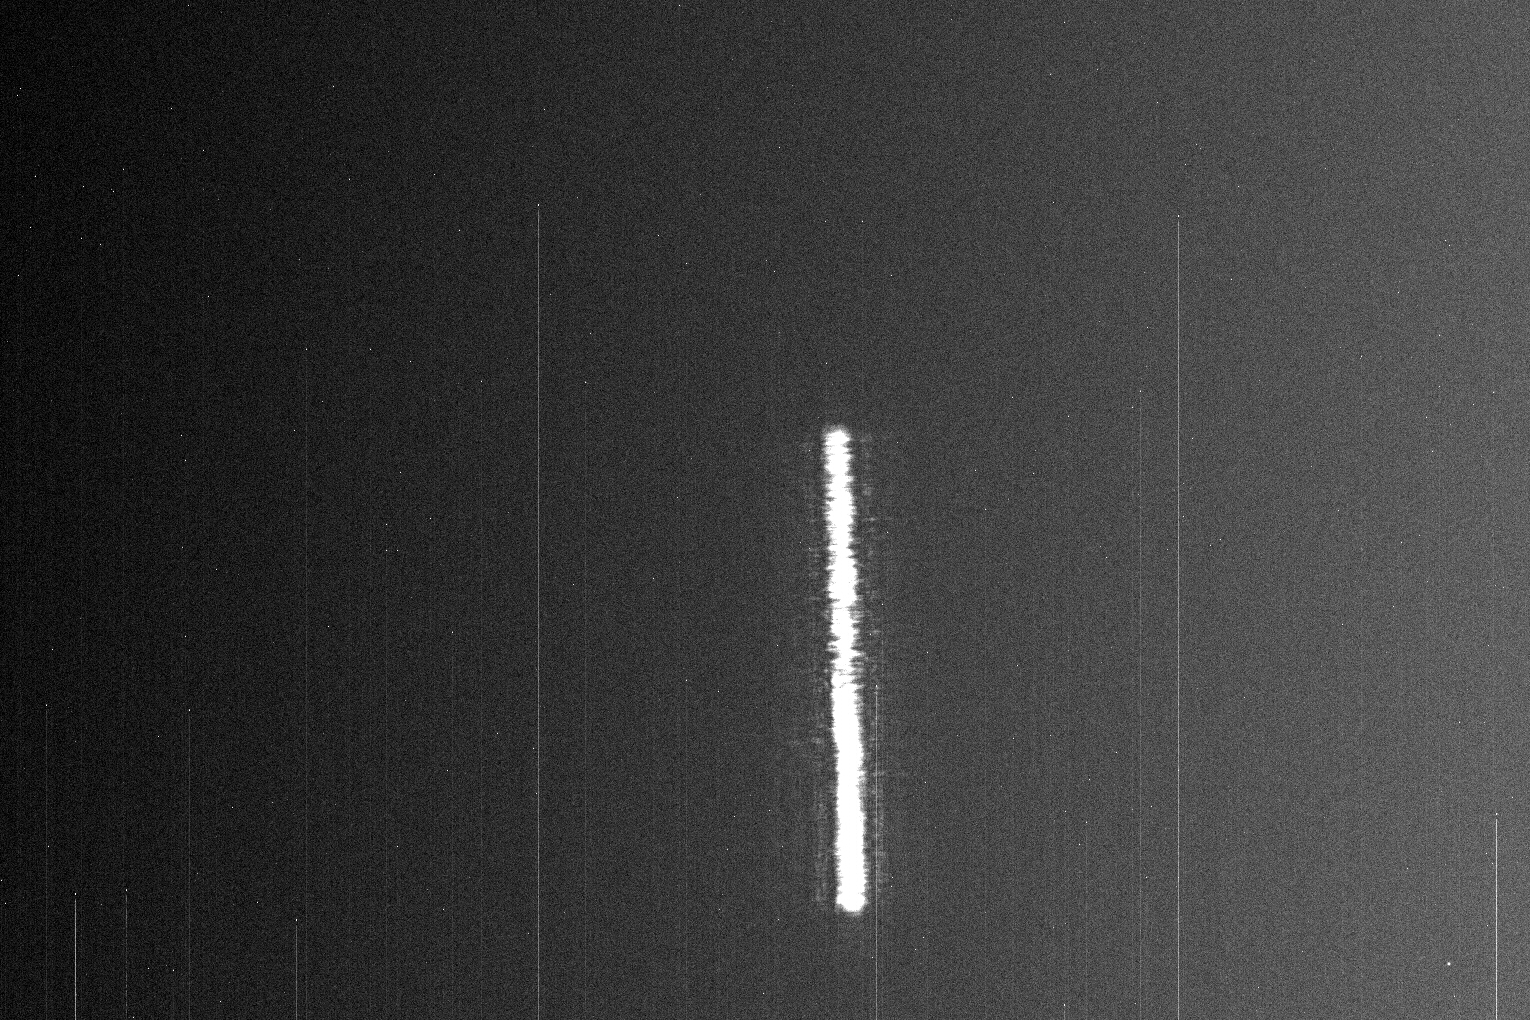
\includegraphics[width=\textwidth]{Daten/spalt_1.jpg}
	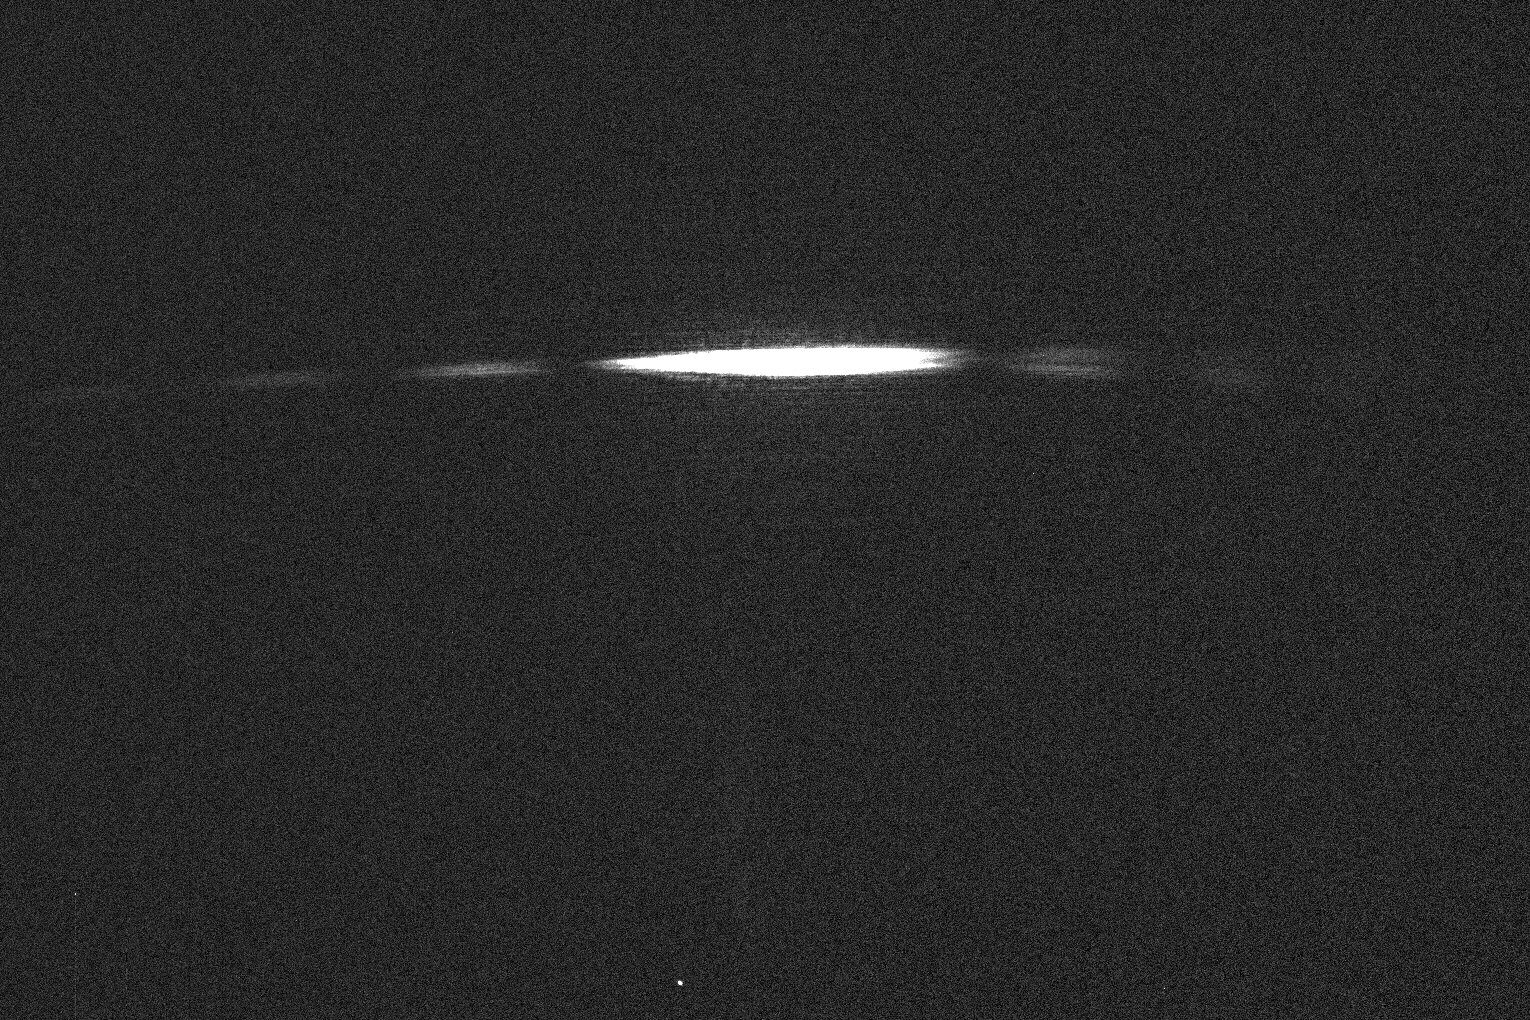
\includegraphics[width=\textwidth]{Daten/spalt_2.jpg}
	\caption[Aufnahme Einzelspalt]{Oben echte Abbildung Einzelspalt. Unten Beugungsbild}
\end{figure}

\begin{figure}[h]
	\centering
	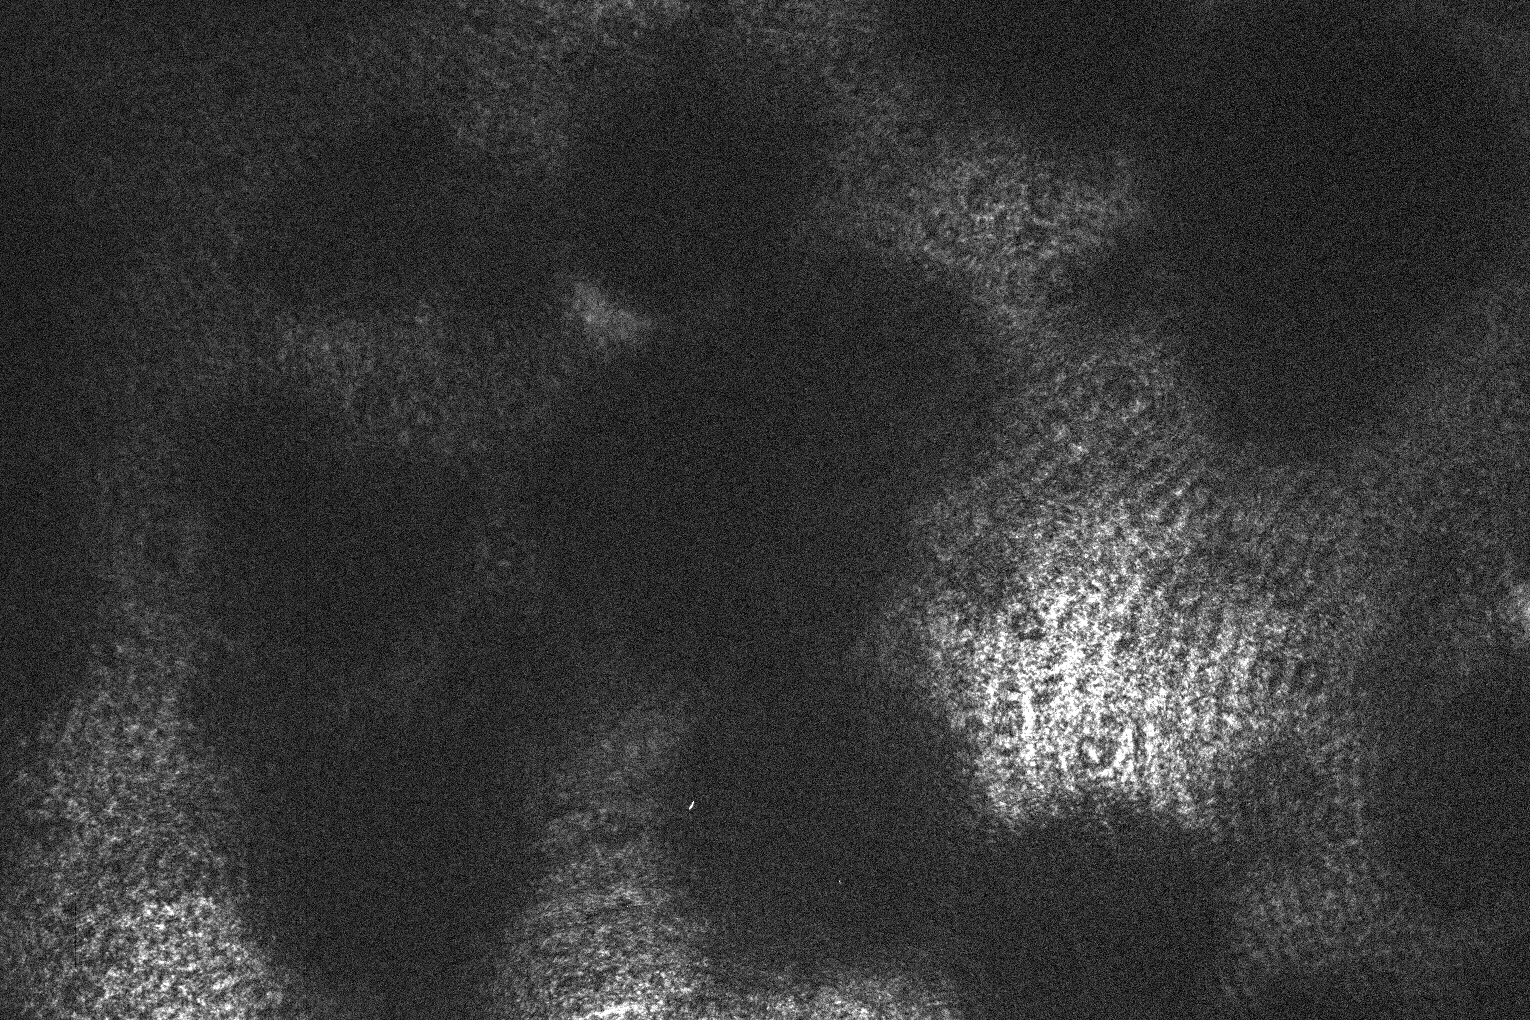
\includegraphics[width=\textwidth]{Daten/bio_1.jpg}
	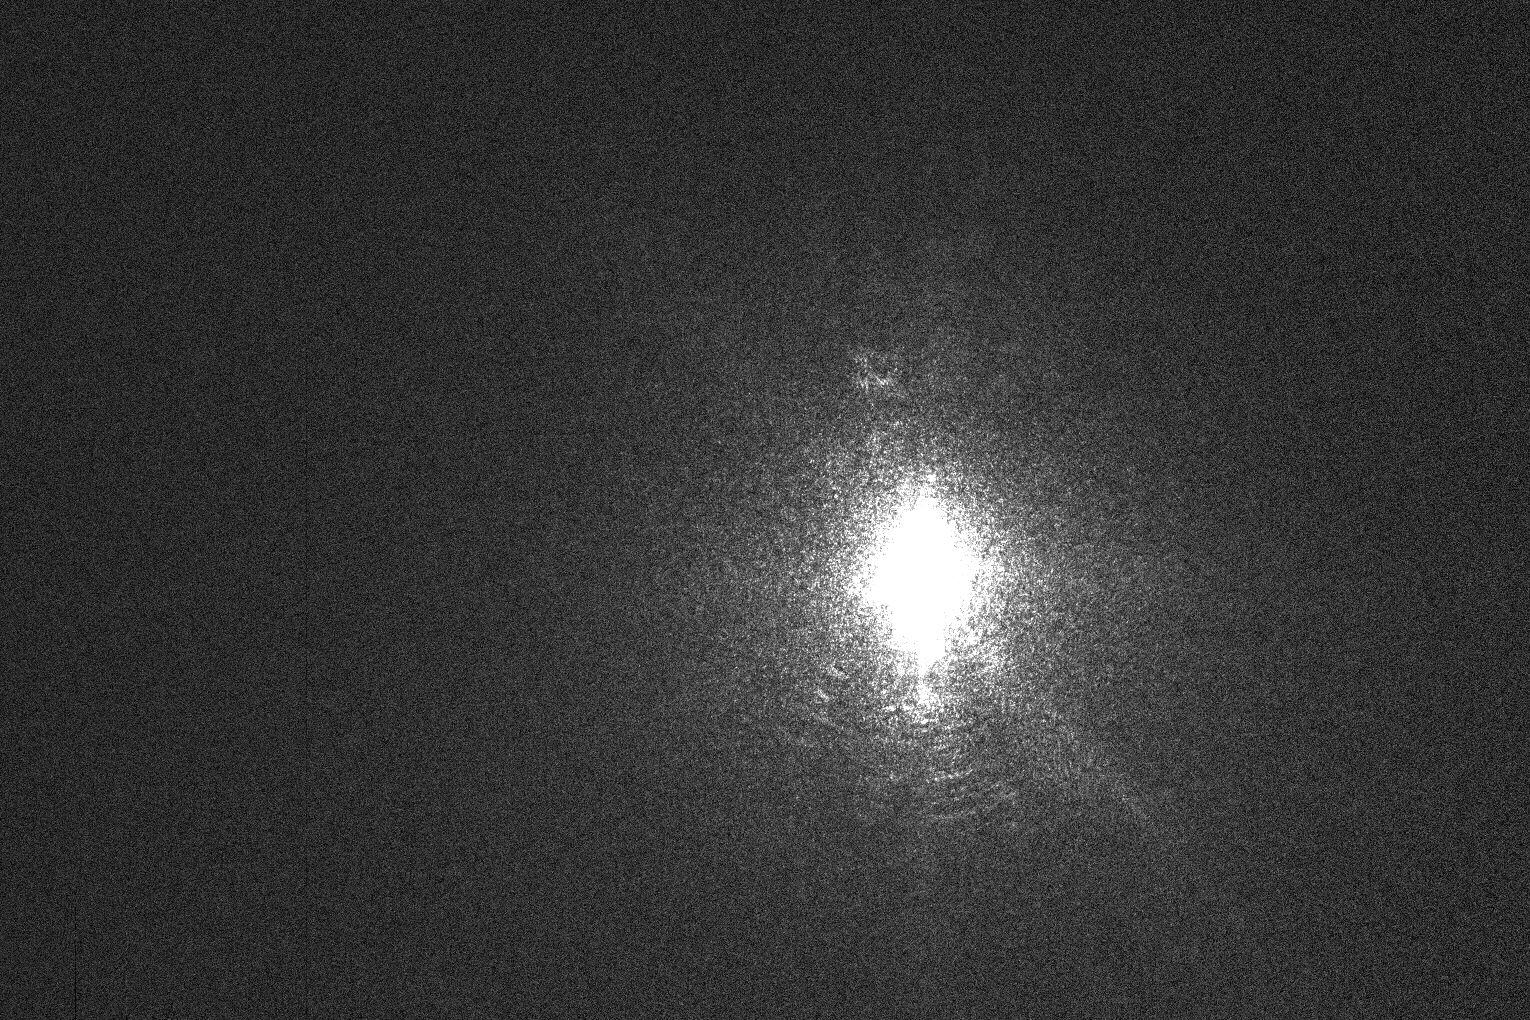
\includegraphics[width=\textwidth]{Daten/bio_2.jpg}
	\caption[Aufnahme biologische Probe]{Oben echte Abbildung unbekannten Probe. Unten Beugungsbild}
\end{figure}
\begin{figure}[h]
	\centering
	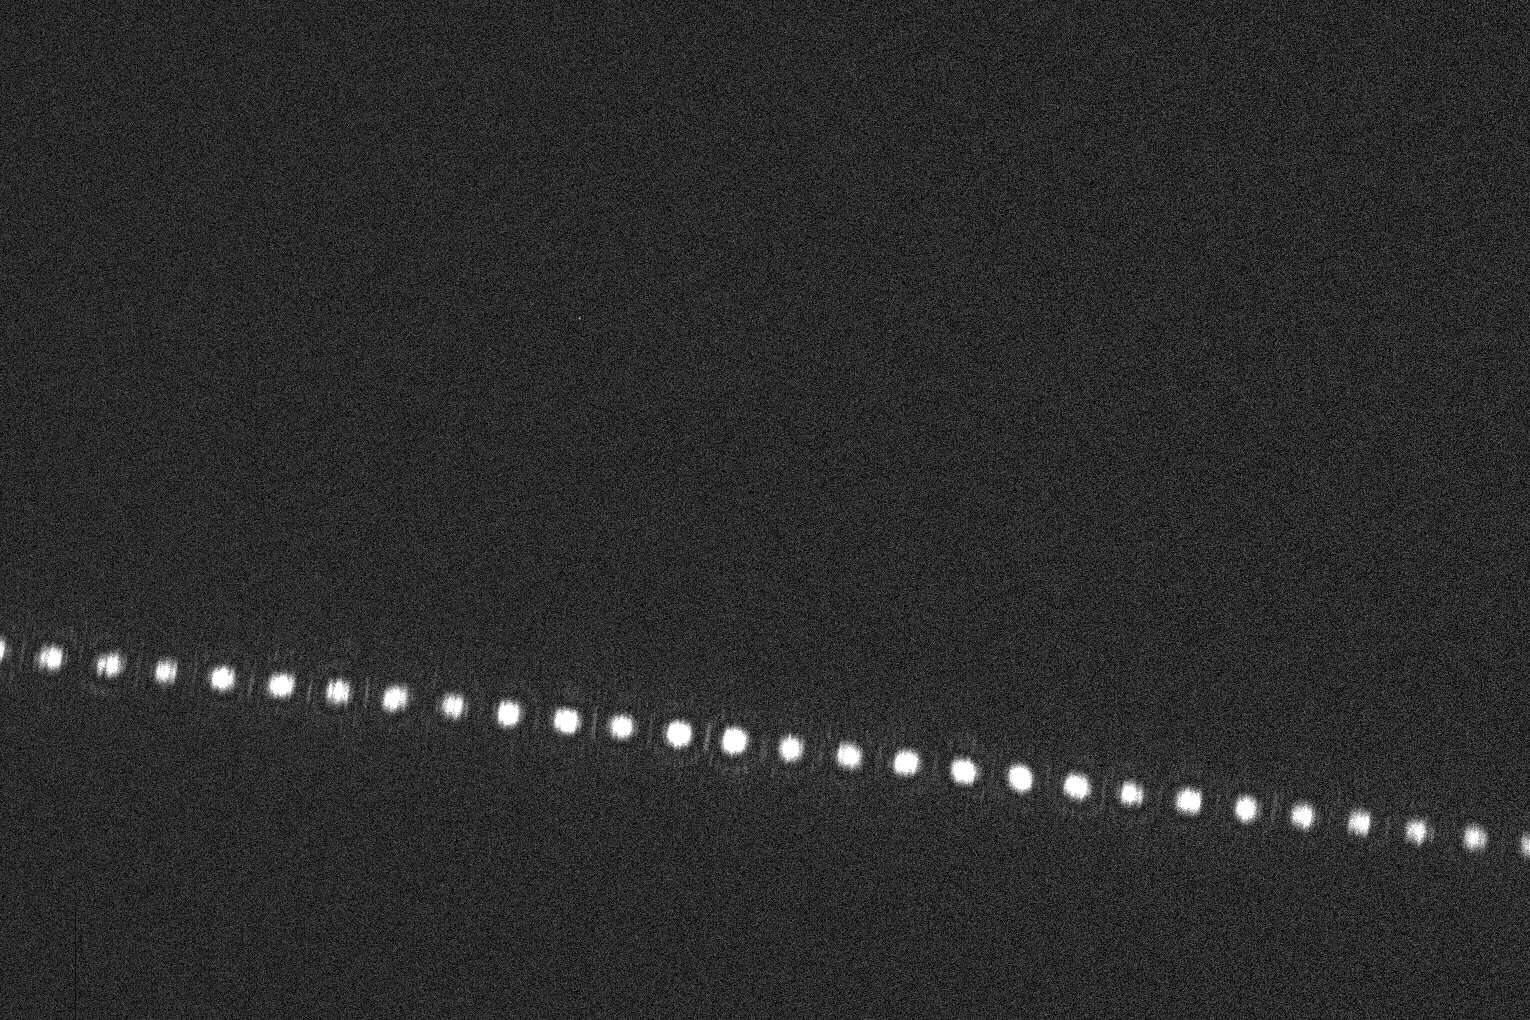
\includegraphics[width=\textwidth]{Daten/gitter_1.jpg}
	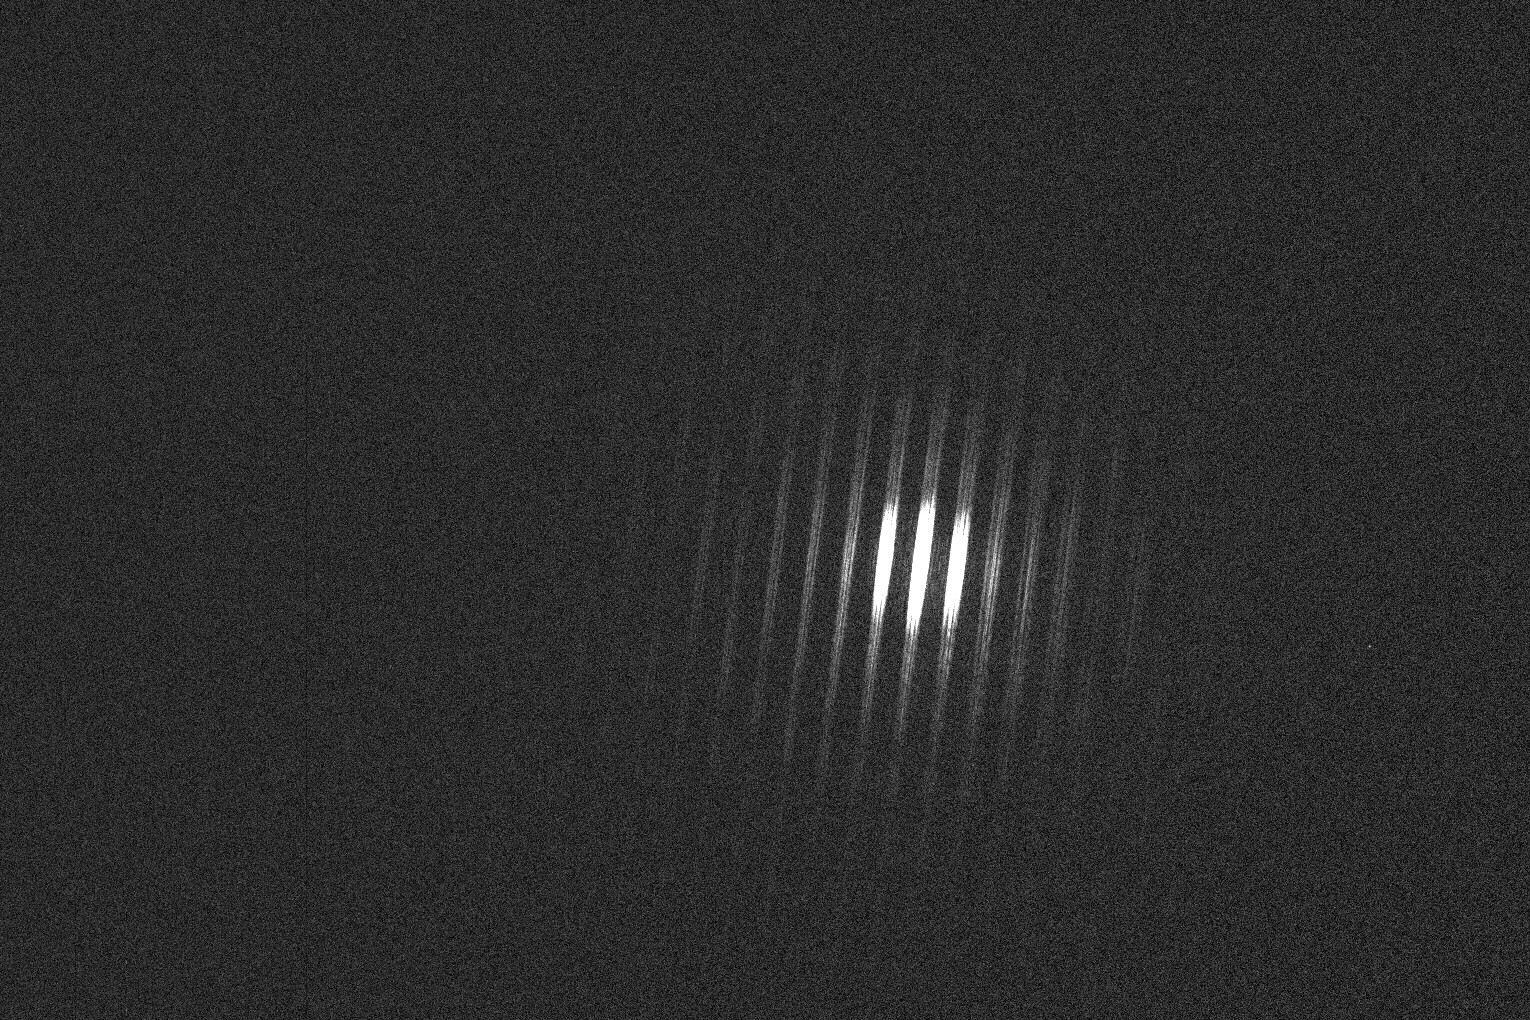
\includegraphics[width=\textwidth]{Daten/gitter_2.jpg}
	\caption[Aufnahme Punktgitter]{Oben echte Abbildung 1-D Gitter. Unten Beugungsbild}
\end{figure}

\begin{figure}[h]
	\centering
	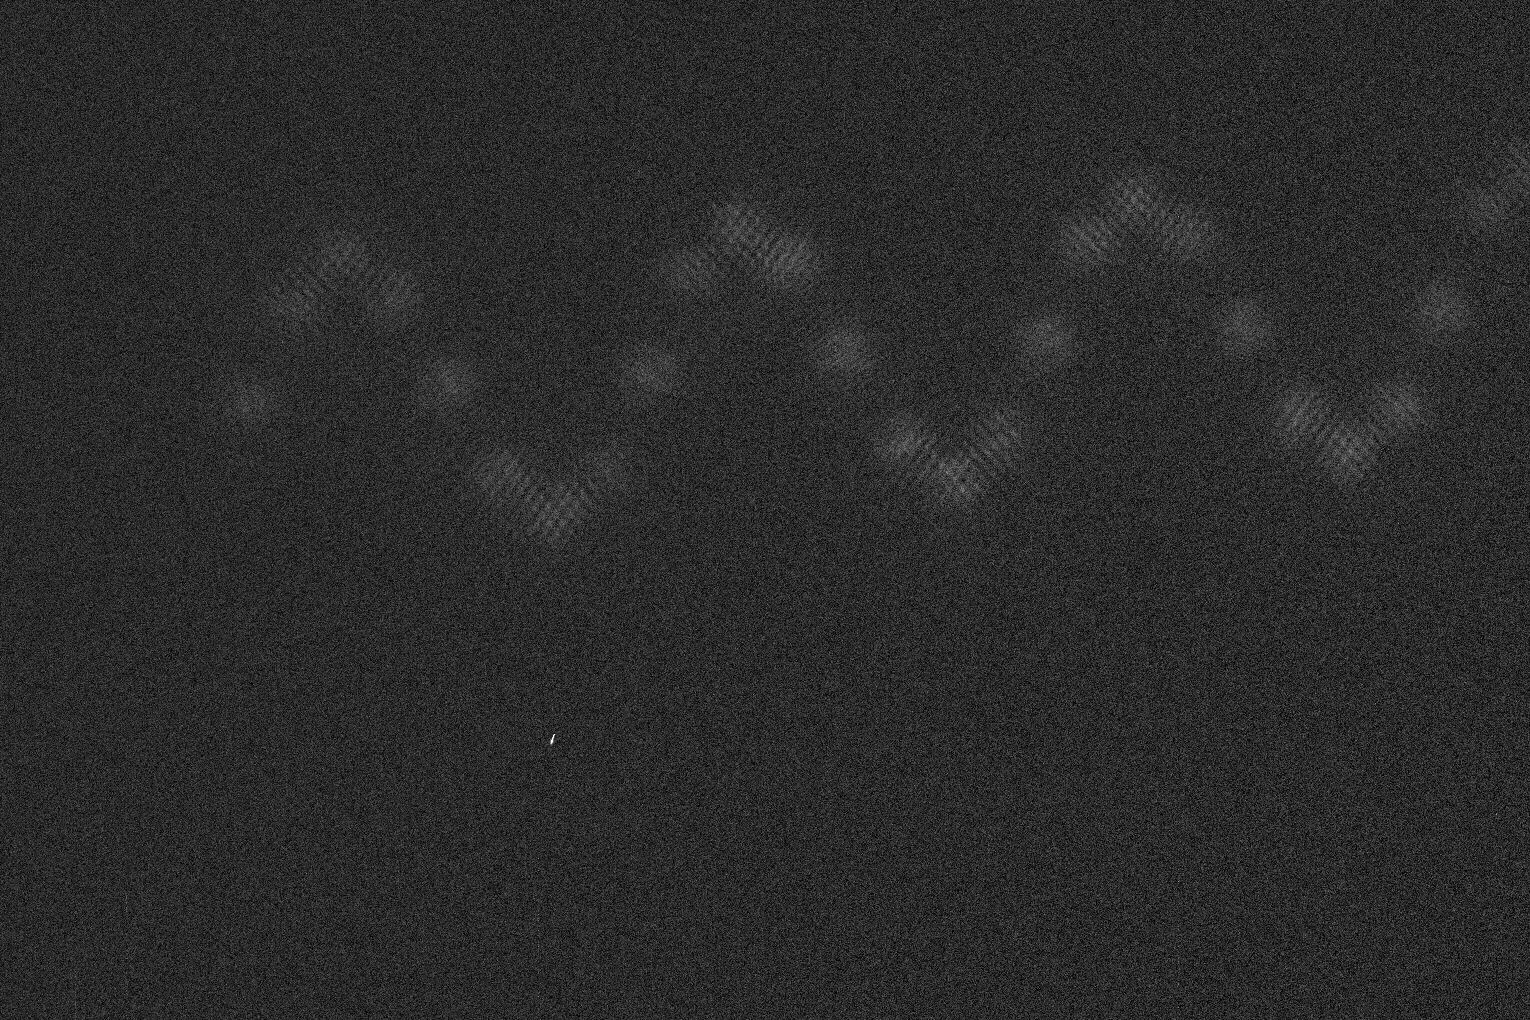
\includegraphics[width=\textwidth]{Daten/sindot_1.jpg}
	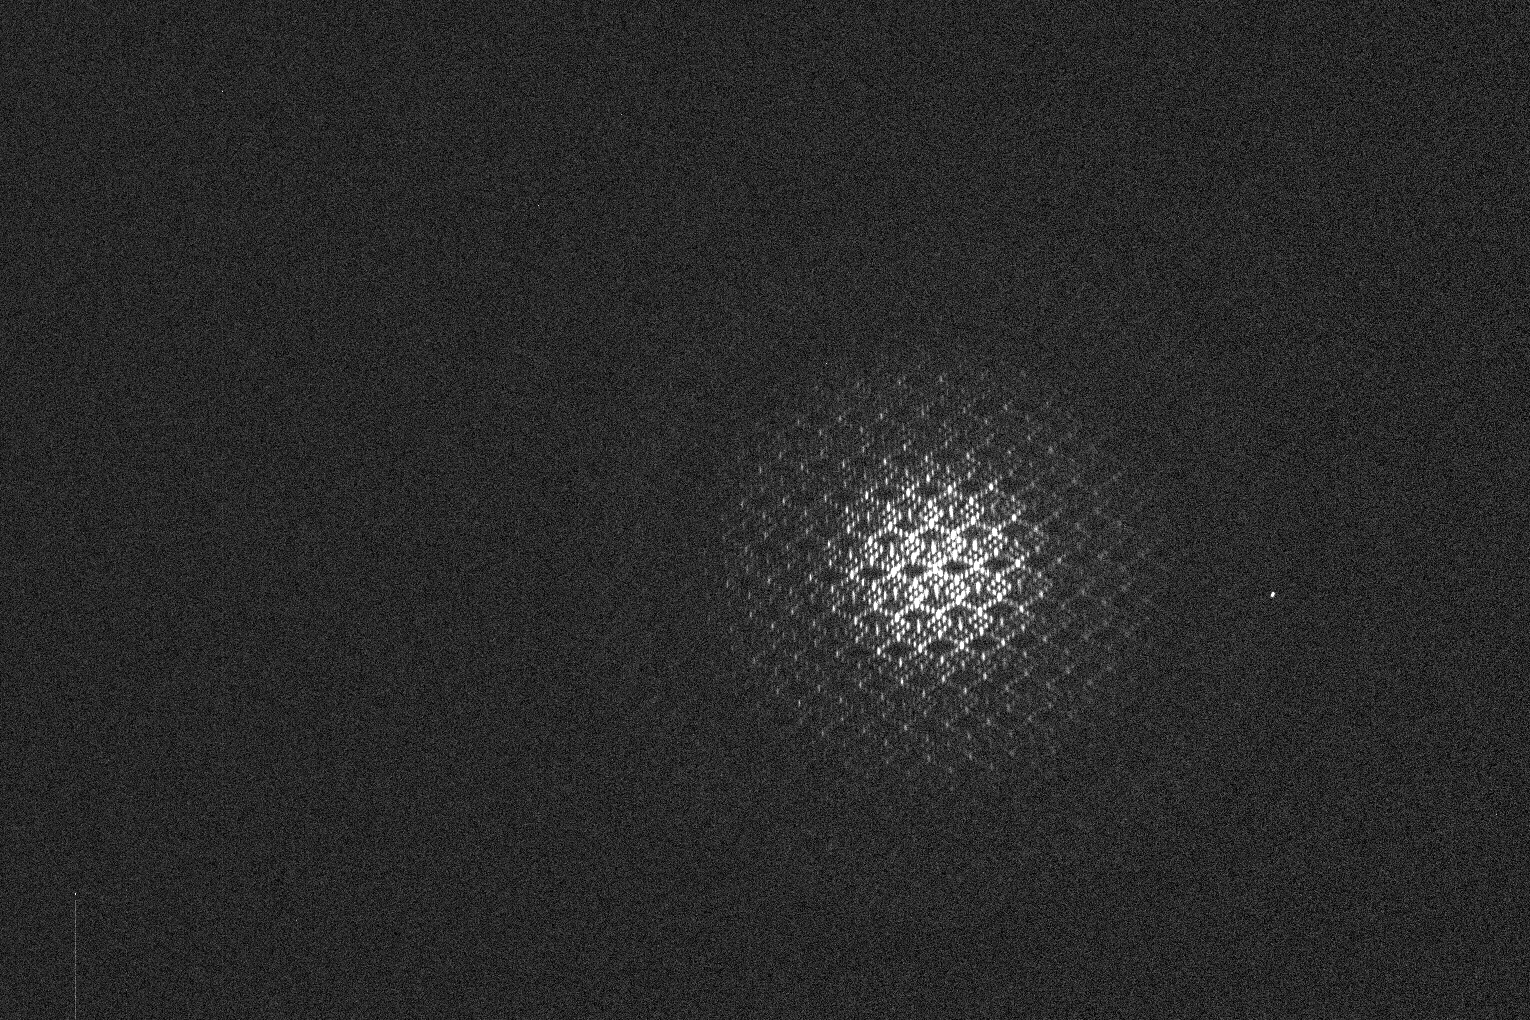
\includegraphics[width=\textwidth]{Daten/sindot_2.jpg}
	\caption[Aufnahme gepunkteter Sinus]{Ob
		en echte Abbildung gepunkteter Sinus. Unten Beugungsbild}
\end{figure}
\begin{figure}[h]
	\centering
	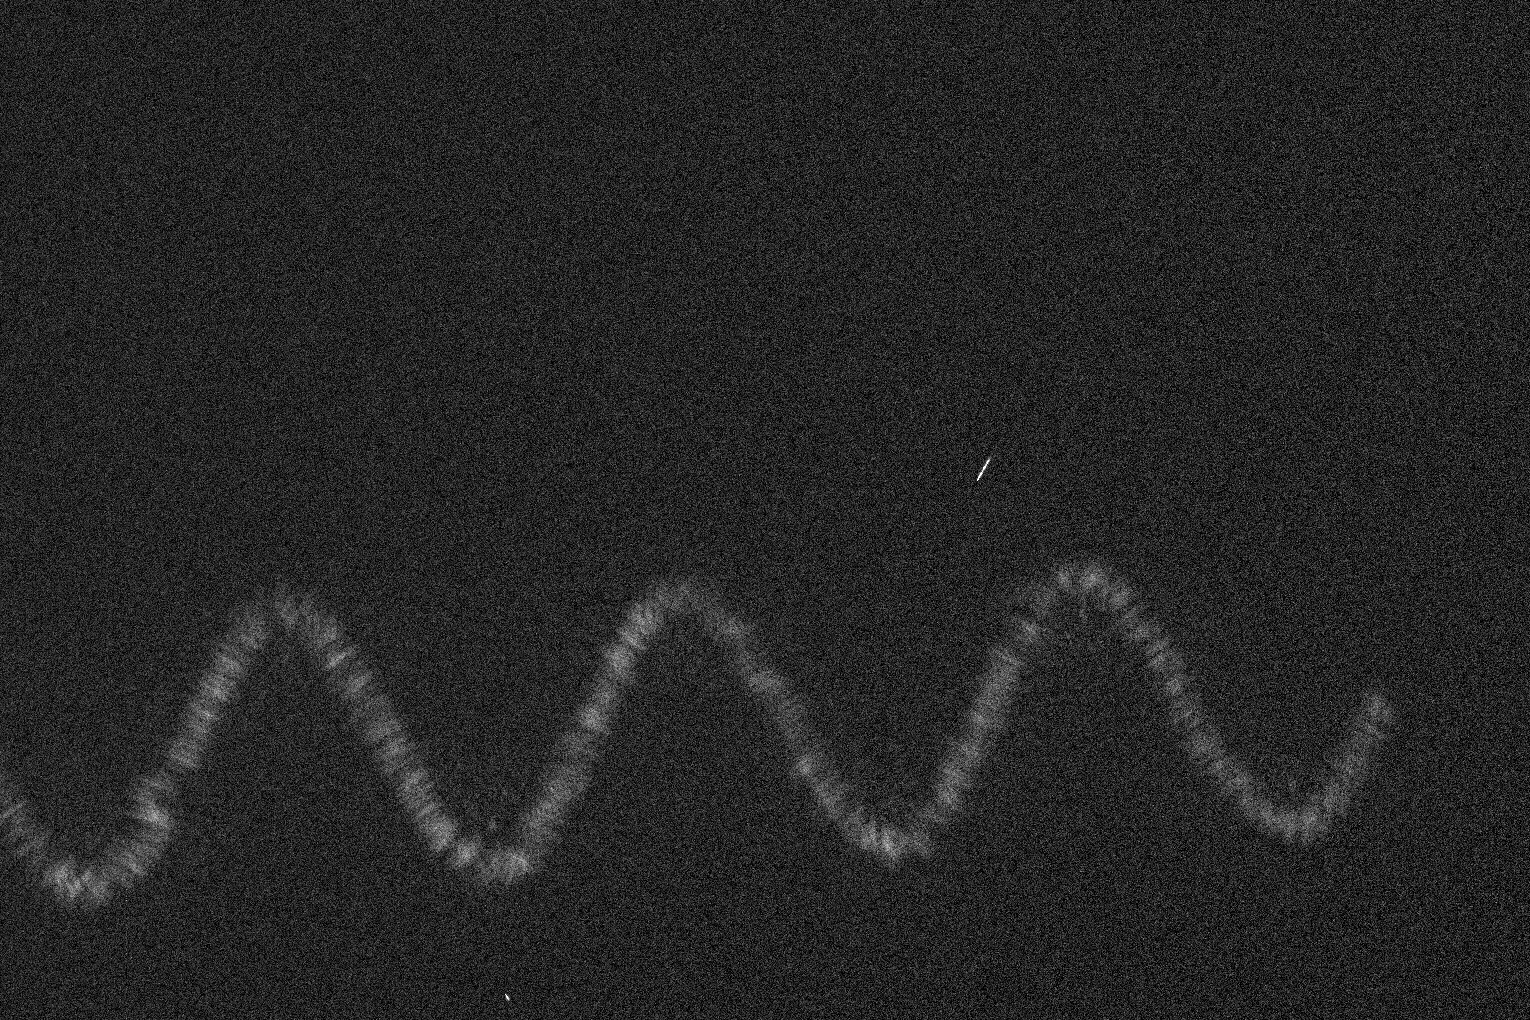
\includegraphics[width=\textwidth]{Daten/sin_1.jpg}
	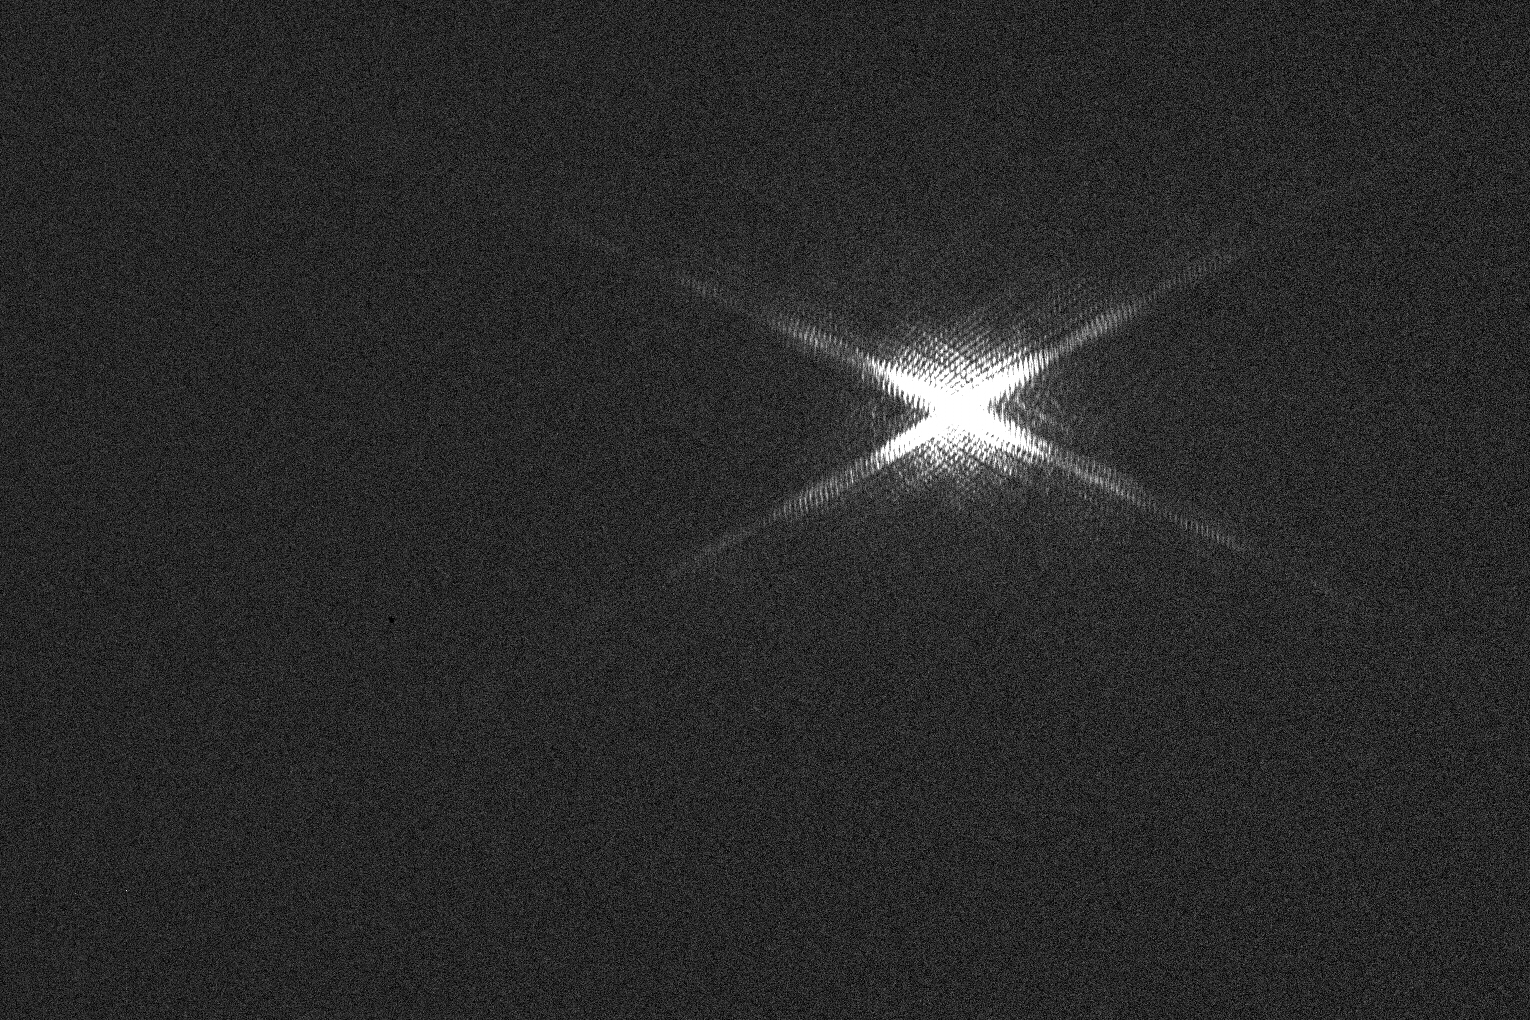
\includegraphics[width=\textwidth]{Daten/sin_2.jpg}
	\caption[Aufnahme Sinus]{Oben echte Abbildung Sinus. Unten Beugungsbild}
\end{figure}
\begin{figure}[h]
	\centering
	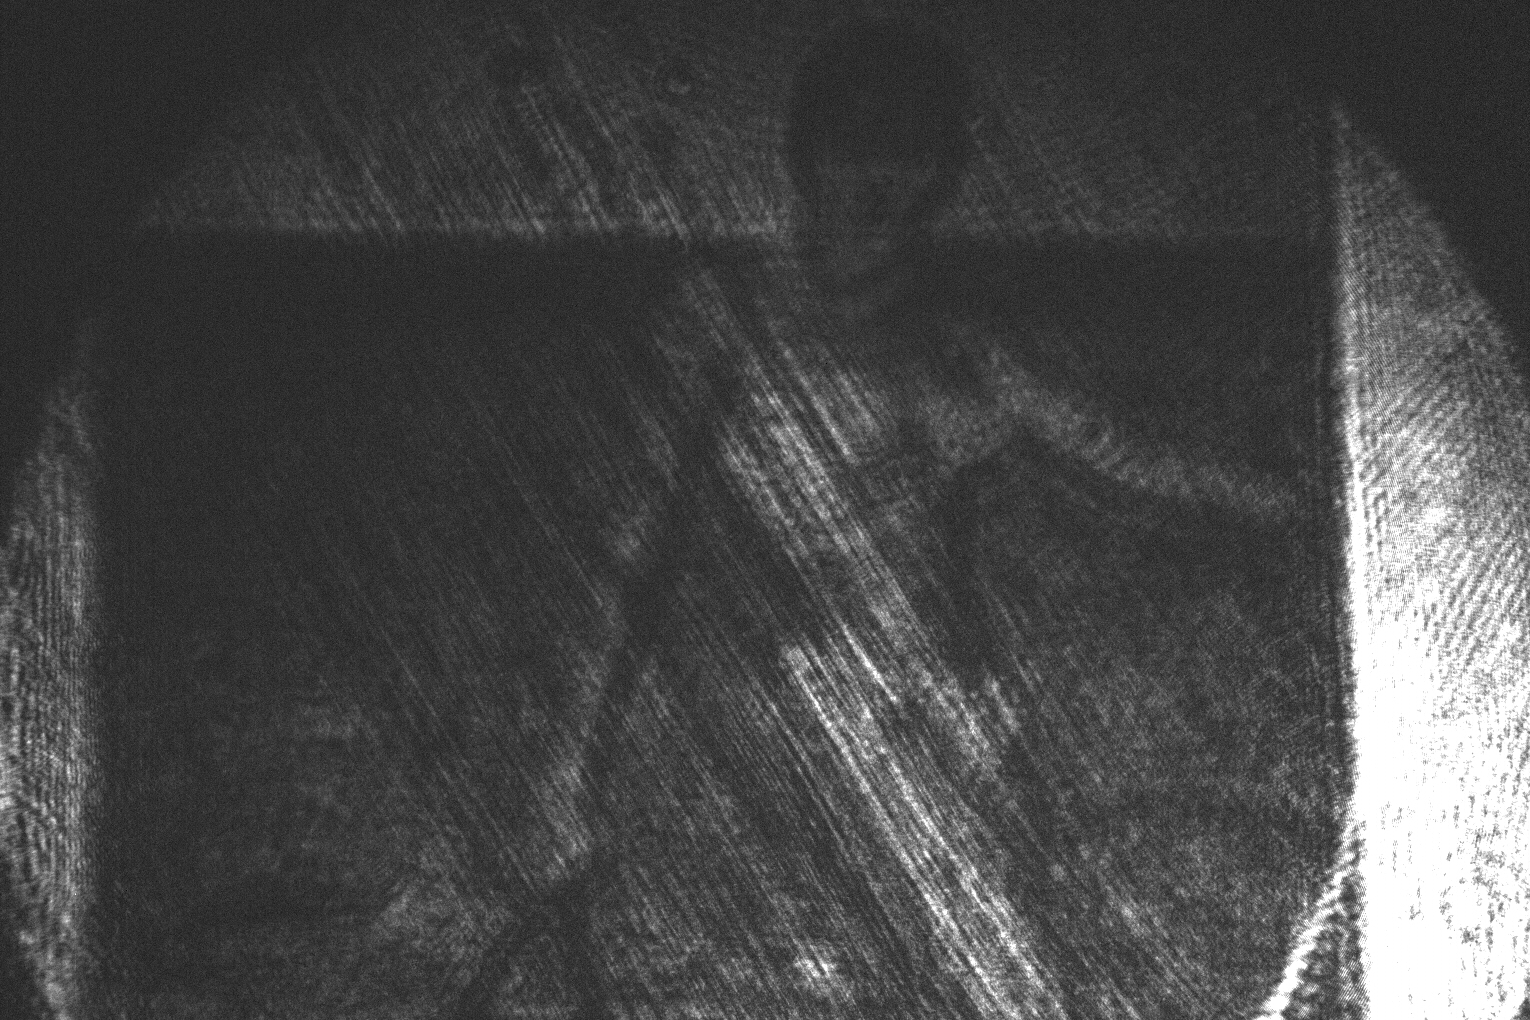
\includegraphics[width=\textwidth]{Daten/frau_1.jpg}
	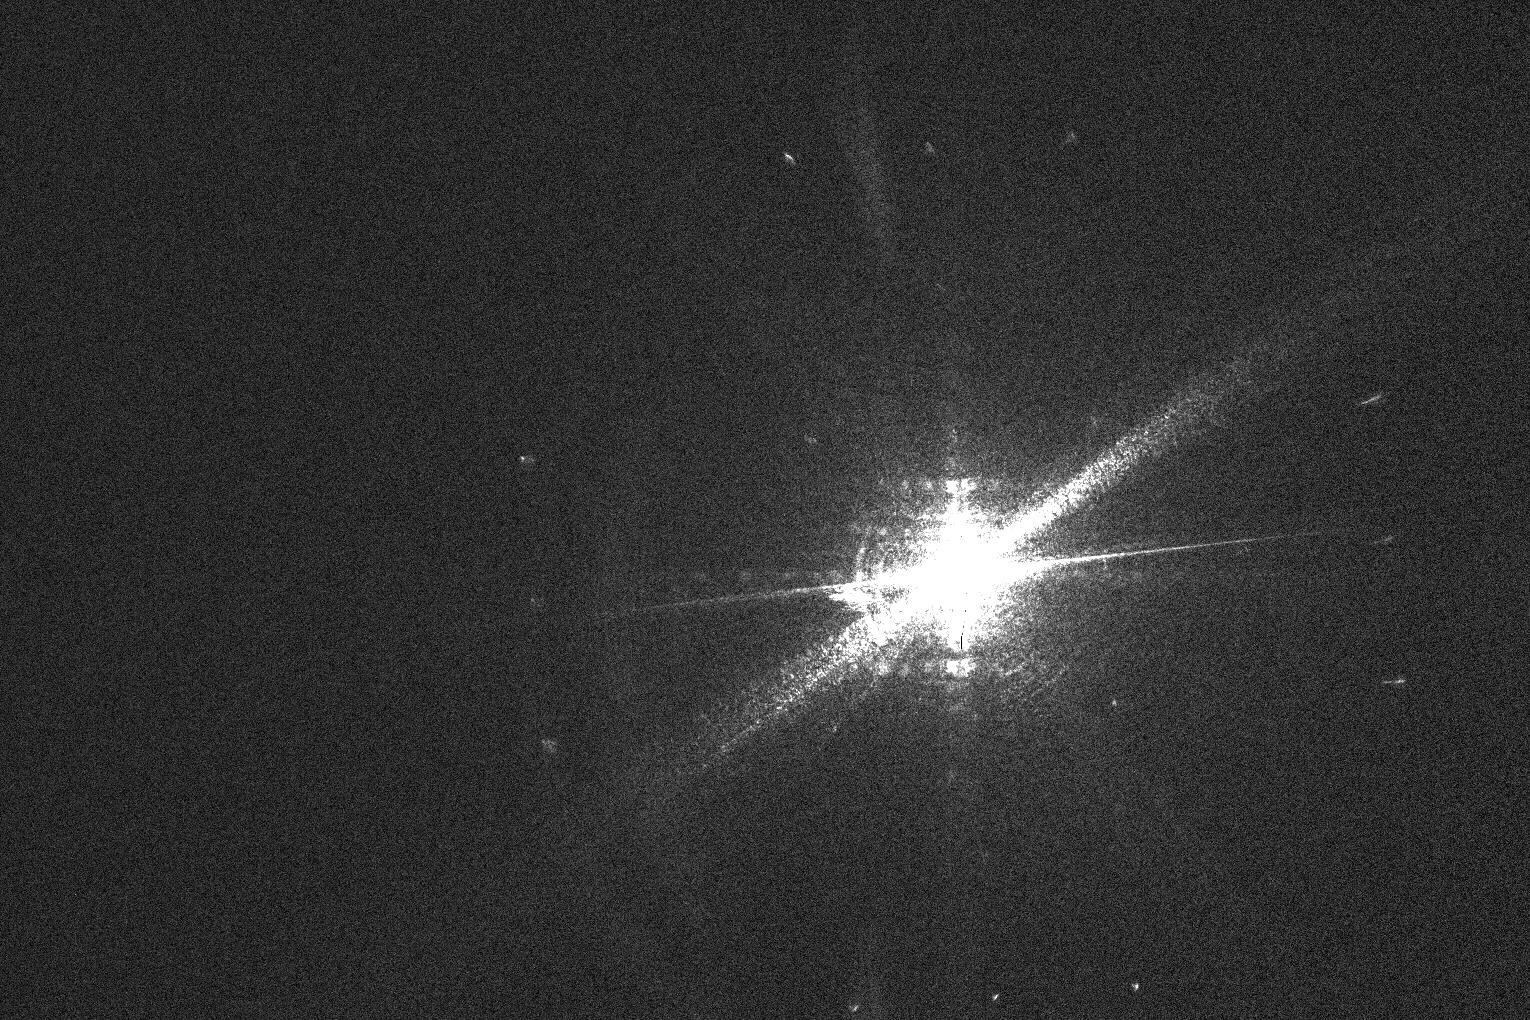
\includegraphics[width=\textwidth]{Daten/frau_2.jpg}
	\caption[Aufnahme Model]{Oben echte Abbildung Bikini Model. Unten Beugungsbild}
\end{figure}
\begin{figure}[h]
	\centering
	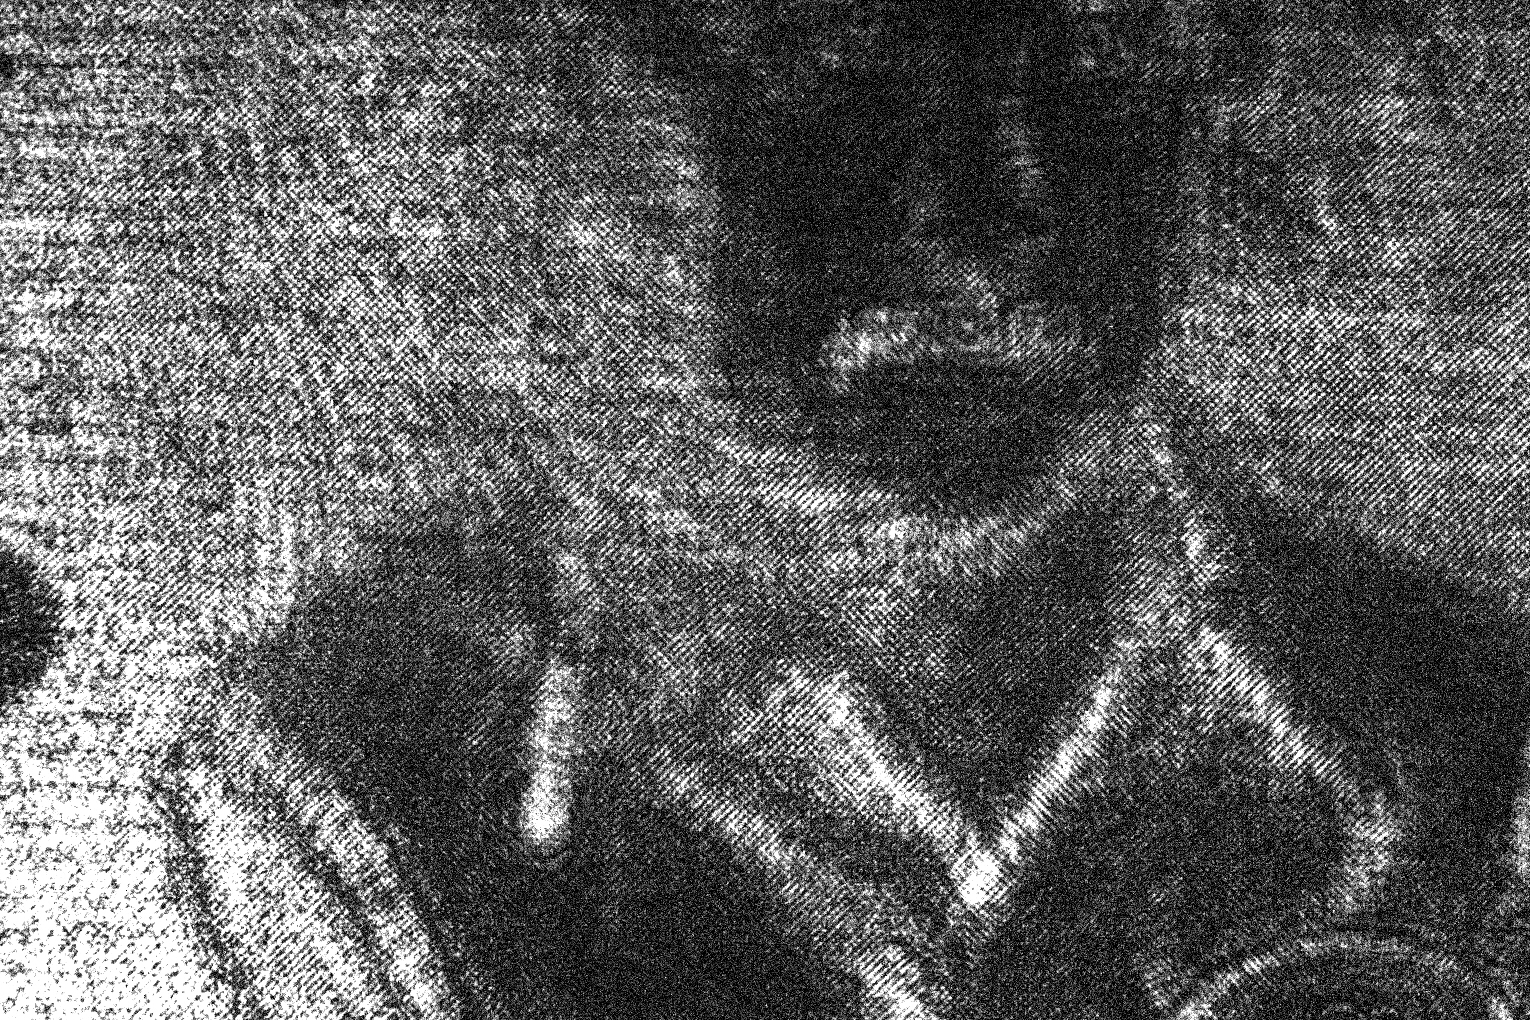
\includegraphics[width=\textwidth]{Daten/einstein_1.jpg}
	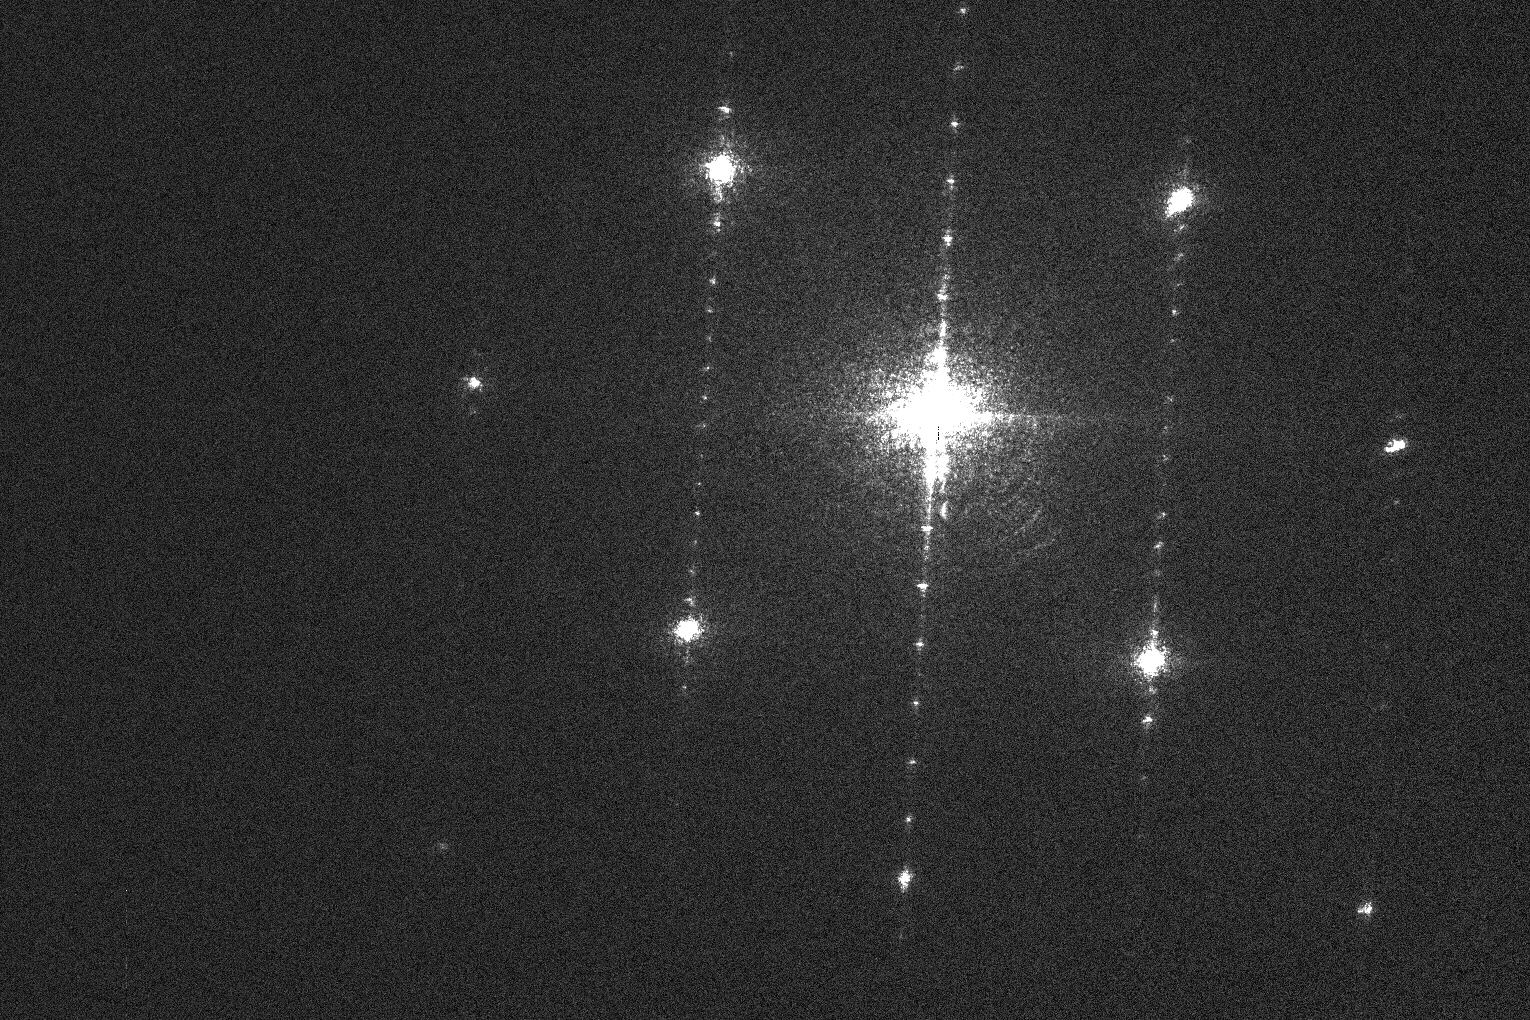
\includegraphics[width=\textwidth]{Daten/einstein_2.jpg}
	\caption[Aufnahme Einstein]{Oben echte Abbildung Einstein. Unten Beugungsbild}
\end{figure}


\begin{thebibliography}{10}
\bibitem{lit:manual} W. Limmer: Anleitung zum Versuch \emph{Hall-Effekt in Halbleitern}. Universität Ulm, Ulm 2014.\\
\url{http://www.uni-ulm.de/fileadmin/website_uni_ulm/nawi.inst.235/Lehre/FP/gesch%C3%BCtzte_Dateien/Anleitung_Halleffekt.pdf}
\bibitem{lit:Iba09} H. Ibach und H. Lüth: \emph{Festkörperphysik}. 7. Auflage, Springer Verlag, Berlin (2009)
\bibitem{lit:Sze07} S. M. Sze und Kwok K. Ng: \emph{Physics of semiconductor devices}. 3. Auflage, John Wiley \& Sons, Inc., New Jersey (2007)
\bibitem{lit:GroMa14} R. Gross und A. Marx: \emph{Festkörperphysik}. 2. Auflage, Walter de Gruyther, Berlin (2014)
\bibitem{lit:Wiki1} Wikipedia-Benutzer Locusta: \emph{Geometriefaktor f für Van-der-Pauw-Methode}. Wikimedia Commons, CC BY-SA 3.0 2010\\ \url{http://commons.wikimedia.org/wiki/File:Pauw_Korrektur.svg}
\end{thebibliography}

\end{document}